\documentclass[11pt,letterpaper]{article}
\usepackage[T1]{fontenc}
\usepackage[utf8]{inputenc}
\usepackage{newtxtext}
\usepackage[margin=1in,headheight=15pt]{geometry}
\usepackage{microtype}
\usepackage{amsmath,amsthm,mathtools}
\usepackage{newtxmath}
\usepackage{booktabs,tabularx,longtable,array}
\usepackage{enumitem}
\usepackage[dvipsnames]{xcolor}
\usepackage{listings}
\usepackage{tikz}
\usetikzlibrary{arrows.meta,positioning,fit}
\usepackage[most]{tcolorbox}
\usepackage{fancyhdr}
\usepackage{hyperref}
\usepackage{bookmark}
\usepackage{needspace}
\hypersetup{colorlinks=true,linkcolor=MidnightBlue,citecolor=MidnightBlue,urlcolor=MidnightBlue,
 pdftitle={GNEISS: Property- and Behavior-Aware Mathematical Elaboration over Lean},
 pdfauthor={OpenAI},pdfsubject={Third-round proof-language proposal}}
\definecolor{ink}{HTML}{16334A}
\definecolor{pale}{HTML}{F1F5F8}
\lstdefinestyle{code}{basicstyle=\ttfamily\small,columns=fullflexible,keepspaces=true,
 breaklines=true,breakatwhitespace=false,showstringspaces=false,
 backgroundcolor=\color{pale},frame=single,rulecolor=\color{black!15},
 xleftmargin=5pt,xrightmargin=5pt,framesep=6pt,aboveskip=10pt,belowskip=10pt}
\lstset{style=code}
\newtcolorbox{designbox}[1][]{colback=pale,colframe=ink,boxrule=.5pt,
 arc=1pt,left=9pt,right=9pt,top=8pt,bottom=8pt,#1}
\newcommand{\code}[1]{\texttt{\detokenize{#1}}}
\newcommand{\Gneiss}{\textsc{Gneiss}}
\newcommand{\N}{\mathbb N}
\newcommand{\Z}{\mathbb Z}
\newcommand{\Q}{\mathbb Q}
\newcommand{\R}{\mathbb R}
\newcommand{\sem}[1]{\llbracket #1\rrbracket}
\newcommand{\EqOn}{\operatorname{EqOn}}
\newcommand{\EqNear}{\operatorname{EqNear}}
\newcommand{\Jet}{\operatorname{Jet}}
\newcommand{\Spec}{\operatorname{Spec}}
\newcommand{\Req}{\operatorname{Req}}
\newcommand{\Obs}{\operatorname{Obs}}
\newcommand{\dom}{\operatorname{dom}}
\newcommand{\id}{\operatorname{id}}
\newcommand{\True}{\mathsf{True}}
\newcommand{\False}{\mathsf{False}}
\newcommand{\Prop}{\mathsf{Prop}}
\newcommand{\Type}{\mathsf{Type}}
\newcommand{\Has}{\mathsf{Has}}
\newcommand{\Contract}{\mathsf{Contract}}
\newcommand{\Respects}{\mathsf{Respects}}
\newcolumntype{Y}{>{\raggedright\arraybackslash}X}
\newcolumntype{P}[1]{>{\raggedright\arraybackslash}p{#1}}
\newtheorem{theorem}{Theorem}[section]
\newtheorem{proposition}[theorem]{Proposition}
\newtheorem{lemma}[theorem]{Lemma}
\newtheorem{corollary}[theorem]{Corollary}
\theoremstyle{definition}
\newtheorem{definition}[theorem]{Definition}
\newtheorem{example}[theorem]{Example}
\theoremstyle{remark}
\newtheorem{remark}[theorem]{Remark}
\setlist{nosep,leftmargin=*}
\setlength{\parskip}{4pt}
\setlength{\parindent}{0pt}
\setlength{\emergencystretch}{2em}
\setcounter{tocdepth}{1}
\clubpenalty=10000
\widowpenalty=10000
\displaywidowpenalty=10000
\AtBeginEnvironment{theorem}{\Needspace{7\baselineskip}}
\AtBeginEnvironment{proposition}{\Needspace{7\baselineskip}}
\pagestyle{fancy}
\fancyhf{}
\fancyhead[L]{\small\textsc{Gneiss}\enspace /\enspace Third-round proposal}
\fancyhead[R]{\small Property-aware mathematical elaboration}
\fancyfoot[C]{\thepage}
\renewcommand{\headrulewidth}{.3pt}

\begin{document}
\begin{titlepage}
\vspace*{.6in}
{\color{ink}\Large THIRD ROUND\quad /\quad PROOF-LANGUAGE DESIGN\par}
\vspace{.45in}
{\color{ink}\fontsize{38}{43}\selectfont\bfseries GNEISS\par}
\vspace{.18in}
{\fontsize{23}{29}\selectfont Property- and Behavior-Aware\par Mathematical Elaboration over Lean\par}
\vspace{.35in}
{\large From proof-carrying answers to\par compositional mathematical contracts\par}
\vspace{.5in}
\begin{designbox}
\textbf{The proposal in one sentence.}\quad Give ordinary Lean terms a second,
proof-producing layer of contextual property types and behavioral signatures,
so that the system reconstructs routine mathematical obligations while preserving
objects, structures, domains, quantifier dependencies, and the author's proof plan.
\end{designbox}
\vspace{.3in}
{\large Prepared for Vladimir Reshetnikov\par}
{\large 6 September 2026\par}
\vfill
\textbf{Status.} This is a research and engineering proposal, not an implemented
proof language. It includes mathematical proofs of a restricted elaboration
calculus and selected contracts, an executed Python acceptance model with 32
passing test methods, and an ordinary-Lean encoding supplied as an uncompiled
specimen. No new Lean kernel, end-to-end frontend, or productivity improvement
is claimed. Repository build and verification results are attributed to their
sources, not presented as reruns performed for this article.
\end{titlepage}

\begin{abstract}
Lean already has the logical expressiveness to state sophisticated mathematical
properties and behavioral constraints. What remains difficult is making those
properties available at the right point in elaboration without repeatedly
repackaging objects, supplying local side conditions, choosing representations,
and navigating theorem interfaces. The two second-round syntheses converge on
an excellent acceptance boundary: a computed answer must carry a proof of the
specified relation to a fixed mathematical object. This article proposes the
next step: use such specifications compositionally \emph{before} the answer is
constructed, as the types of mathematical operations and the constraints that
guide synthesis.

\Gneiss{} separates an ordinary carrier type, an evidence-backed contextual
property view, and a behavioral contract describing what an operation preserves
or requires. It makes proof-valued inference routine while keeping data,
structures, branches, and witness dependencies explicit. A bidirectional
elaboration calculus translates into ordinary Lean declarations; observation
contracts govern finite truncation, locality, precision, and representation
changes. Worked examples cover triangular-kernel inversion, local iterated
derivatives, the semistable-modularity proof architecture and Frey-model exact
division in the FLT repository, and a polynomial certificate checker with an
explicit denotation theorem. Leant is integrated as an untrusted structural
candidate producer, with its existing behavioral machinery and trust boundaries
preserved. Genuine kernel extensions are assessed separately from conservative
surface-type extensions. The outcome is a narrow implementation agenda with
falsifiable evaluation criteria rather than another assertion that familiar
notation alone will shorten proofs.
\end{abstract}

\clearpage
\tableofcontents
\clearpage

\section{The decision: enrich the elaboration type system first}

\subsection{What should become easier}
A mathematician says ``let $x$ be positive,'' uses its nonzeroness when dividing,
uses positivity again when preserving a strict inequality, and does not rename
$x$ each time. A mathematician says ``differentiate this identity on the open
set,'' carrying the domain through the argument without restating a neighborhood
lemma at every point. An algebraist passes to a finite matrix presentation,
uses a theorem about square matrices, and knows precisely which observation of
the original operator that theorem establishes.

These are not requests for less rigor. They are requests for a better interface
to \emph{persistent mathematical information}. The author supplies the conceptual
step; an elaborator should reconstruct its routine premises, explain the
remaining ones, and retain a proof of the exact result.

\begin{designbox}
\textbf{Three layers, three different questions.}

\textbf{Carrier:} What object is this?\quad
$x:A$, or $f:A\to B$.

\textbf{Property view:} What has been proved about this very object in this
context?\quad $P(x)$, continuity on $U$, squarefreeness of $N$.

\textbf{Behavioral contract:} What does an operation require and preserve?\quad
A relation between its input, output, domain, observation, and any selected data.
\end{designbox}

The second layer does not construct a new mathematical $x$. The third layer is
not merely a description of the output's shape: it relates that output to the
particular input. A sorting function must preserve the input multiset, not just
return a sorted list. A matrix presentation must represent the specified
operator, not an isomorphic but unrelated object. A finite jet must be the jet
of the retained series, not merely a polynomial satisfying some nearby equation.

\subsection{An extension, but not initially an extension of logic}
There are two meanings of ``extend Lean's type system.'' One is to add primitive
kernel rules, perhaps changing conversion or the logical meaning of a type. The
other is to enrich the types that authors write and that elaboration checks,
translating those types into the existing dependent type theory.

\textbf{\Gneiss{} proposes the second as its first implementation.} This is a real
extension of the user-facing static discipline: function application, property
inference, and observation selection generate typed obligations according to
new rules. It is not a claim that Lean lacks subtypes, dependent products, or
proof-carrying structures. Lean's existing \code{Subtype} already pairs a value
with a proposition's proof and erases that proof in compiled representations
\cite{lean-subtypes}. The target is the \emph{elaboration and reuse} of such
information, not its logical expressibility.

A subsequent kernel extension would need a separate argument for its benefit.
Section~\ref{sec:kernel} evaluates the possibilities. In particular, arbitrary
CAS equality and arbitrary semantic subtyping should not become definitional
equality merely to save explicit transports.

\subsection{What is distinctive relative to round two}
The earlier designs already have guards, typed results, observation relations,
method wrappers, and precision planning. \Gneiss{} does not rename those as new
inventions. Its proposed increment is a \emph{single operational discipline}
connecting them: a property view is an input to bidirectional elaboration, and
a behavioral signature transfers those views across a mathematical expression
or proof step. Both theorem application and verified computation implement that
same signature. The author can inspect the resulting obligations as a compact
mathematical type, rather than as an accidental sequence of tactic subgoals.

The decisive experiment is therefore not ``does the syntax look shorter?'' It
is whether type-directed property and behavior inference removes interventions
that an equally equipped Lean library and tactic interface do not already
remove, while preserving statement comprehension.

\section{What the source material establishes}\label{sec:reading}

\subsection{Reading scope and version discipline}
Both requested round-two syntheses were read closely, including their comparison,
corrections, worked contracts, negative cases, implementation recommendations,
and questions for round three. They were read at Brainstorm commit
\code{b052ec011beb96a7c48df2a9988823f0f779b445}. The first report is
\emph{Mathematical Objects, Certified Computation}; the second is
\emph{Nine Workbenches} \cite{syn-a,syn-b}.

Their revision relationship matters. The current second report explicitly accepts
several criticisms of its earlier version. It no longer claims that nobody
mentioned \code{grobner}, that a witness plus coverage establishes a complete
solution set, or that a nondegenerate timing experiment proves general checker
scalability. The first report's historical criticisms should not be restated as
unrepaired defects in the current second report.

Representative Lean sources were also read directly. The ProveIt sample includes
\code{BinomialInversion.lean}, the autonomous-derivative development, and
\code{TriangularKernelInverse.lean} \cite{binomial,autonomous,triangular}.
The FLT sample includes the Frey-package definition and the mathematical body
of semistable-model modularity. The Leant review covers its verification
boundary, engine interface, and synthesis/behavioral handoff documentation.
Appendix~\ref{app:sources} records exact revisions and file locations. This is
a focused architectural reading, not an audit of every file, a rerun of the
FLT build, or a proof-length census.

\subsection{The inherited commitments}
The syntheses agree on the essential logical boundary. A request fixes an input
$i$, an output family $O(i)$, and a specification; an accepted answer consists of
\[
                 o:O(i),\qquad p:\Spec(i,o).
\]
The relation can be equality, equality on a domain, an enclosure, a finite jet,
a witness property, or complete characterization of a solution predicate. These
are not interchangeable badges. Each promotion needs a theorem with all its
premises \cite{syn-a,syn-b}.

Other commitments are equally important: retain the original object; bind guards
in ordered dependent contexts; distinguish proof-producing search from acceptance;
replay the exact proposed edit; keep retained evidence available without the
discovery service; and compare any new frontend with ordinary Lean supplied
with the same libraries and services. All remain part of \Gneiss.

What should \emph{not} be inherited is the temptation to surround that boundary
with a large speculative language before demonstrating a useful workflow. The
syntheses rightly ask for a proved checker and concrete obligations. The present
article answers with a restricted calculus, complete paper proofs of its local
contracts, an executable acceptance model, and a precisely scoped Lean
implementation target. It does not substitute these for an actual compiled
frontend or claim that the last engineering step is automatic.

\subsection{A crosswalk rather than a novelty score}
\begin{center}\small
\begin{tabularx}{\textwidth}{@{}P{1.38in}YY@{}}
\toprule
Round-two contribution & Kept in \Gneiss{} & Proposed additional work\\
\midrule
Locus's property/guard workspace & Contextual evidence and ordered dependencies & Make the evidence part of bidirectional term checking; measure the index against Lean's local context.\\
Concord's demand-indexed jets & Backward precision requests & Generalize to typed observation-transfer signatures, including domains and finite sections.\\
Meridian's result properties & Theorem-backed implications, not a total strength ranking & Use implication evidence for argument checking and specification subsumption.\\
Facet and Vantage's representations & Exact presentations separate from observations & Require operation-specific respectfulness before substituting a representation.\\
Prism's delegated construction & A fixed specification may authorize witness search & Distinguish input-dependent contracts from proof-only refinement inference.\\
Accord's validation states & Candidate, checked result, replayed result remain distinct & Render inferred property views without upgrading their validation status.\\
Noema's circular-guard restriction & A result cannot establish its own prerequisite & Enforce a dependency-stratified rule interface in the acceptance model.\\
\bottomrule
\end{tabularx}
\end{center}
These attributions follow the detailed cross-reviews in the syntheses
\cite{syn-a,syn-b}. They are not claims that these ideas have no earlier history.
Refinement sorts and proof-irrelevant interpretations, in particular, have
substantial prior art \cite{lovas-pfenning}.

\section{A diagnosis grounded in actual Lean code}\label{sec:diagnosis}

\subsection{Do not confuse three kinds of verbosity}
The source examples show at least three distinct costs. \emph{Mathematical work}
includes inventing an induction invariant, proving kernel orthogonality, or
assembling a modularity argument. \emph{Interface work} includes transporting a
known identity through a finite presentation, finding a theorem's correct local
hypotheses, and passing a witness's properties to the next theorem.
\emph{Generated engineering text} includes repetitive environment configuration
and pipeline names. A proposed language must not claim the same remedy for all
three.

The FLT modularity proof file has extensive generated instance/simplification
configuration before the mathematical body. Its README explicitly describes the
sources as machine-generated and written primarily for checking. Those long
configuration lines are not evidence that every human-written Lean proof needs
that boilerplate. Conversely, hiding them in a renderer is not a mathematical
automation breakthrough \cite{flt-readme,flt-modularity}.

\subsection{Local analysis: information is present, but must be routed}
In \code{AutonomousIteratedDeriv.lean}, the induction step establishes an
identity near $x$ from an identity on an open set, transfers the derivative
through that eventual equality, applies the chain rule, and uses the recurrence
for a derivative family. The actual statement asks for differentiability only
at values in $W(s)$, not globally \cite{autonomous}.

The recognizable mathematical sentence is ``differentiate the induction
identity on $s$.'' That sentence is sound only when its type carries the domain
and local equality relation. A type-directed elaborator should reconstruct the
neighborhood step from $x\in s$ and openness of $s$, but must not manufacture
global smoothness or a pole-avoiding branch. This example is not a reason to
replace a compact existing theorem by a longer narrative. It is a reason to
make that theorem's locality contract easy to invoke and compose.

\subsection{Finite algebra: the representation has a behavioral precondition}
In \code{TriangularKernelInverse.lean}, a kernel becomes a finite square matrix
by zeroing its upper triangle. A matrix-product entry is identified with an
interval convolution. One-sided inverse commutation is then applied to the
finite matrices, and an entry is transported back to the kernel
\cite{triangular}.

A naive frontend might summarize this as ``one-sided inverses commute.'' That
is false for arbitrary endomorphisms of infinite-dimensional spaces. The
missing information is not a scalar side condition: it is the fact that the
operators admit compatible finite square presentations. Section~\ref{sec:triangular}
turns this into a behavioral property, rather than an unstructured automation
hint.

\subsection{Arithmetic geometry: witnesses carry a changing collection of laws}
The semistable-modularity body chooses a residual level, registers that level as
nonzero, passes several level conditions to a lifting theorem, and, in the other
branch, chooses a different curve $W'$ together with a relation to $W$. Later it
extracts a squarefree level $N$ and derives the square- and cube-divisibility
exclusions needed by the next lifting theorem \cite{flt-modularity}.

Much of this is already sensible Lean. The genuinely reusable opportunity is
\emph{property propagation at a selected witness}: positivity yields nonzeroness;
squarefreeness yields prime-power exclusions; an exact-conductor-level package
forgets to a weaker modular-model package. The curve $W'$ itself cannot be
silently identified with $W$. Its transfer relation has a different meaning from
equality and must remain visible.

\subsection{Lean has already done some of the bundling}
\code{FreyPackage} bundles $a,b,c\in\Z$, their nonzeroness, a prime exponent
$p\ge5$, the Fermat equation, coprimality, and the congruences used to normalize
the model. Helper theorems derive additional consequences
\cite{frey-package}. Replacing this structure with another record and claiming
that properties have finally become types would miss the point.

\Gneiss{} must work with this existing object. It should expose its facts as
contextual evidence, derive only the consequences demanded by a subsequent
operation, and preserve the exact interpretation of the integer and rational
curve definitions. The same principle applies to existing continuous maps,
linear maps, equivalences, and other bundled interfaces.

\subsection{Binomial inversion: a property of two whole sequences}
The binomial-inversion file gives a useful warning against overaggressive
property inference. Its module-valued theorem requires only an additive
commutative group $M$, with integer scalar action, not a field or a
$\Q$-algebra. For $a,b:\N\to M$, it relates the two \emph{universal} properties
\[
 \forall n,\quad b_n=\sum_{k=0}^n\binom nk\mathbin{\cdot}a_k,
 \qquad
 \forall n,\quad a_n=\sum_{k=0}^n(-1)^{n-k}\binom nk\mathbin{\cdot}b_k,
\]
where the dot denotes integer scalar action. The source proves an equivalence
between these whole-sequence properties \cite{binomial}.

It does not assert an equivalence row by row under only the row-$n$ premise.
For example, over $\Z$, take $n=1$, $a_0=a_1=0$, $b_0=1$, and $b_1=0$.
The row-$1$ forward identity holds, but the purported inverse row would say
$0=b_1-b_0=-1$. A property view saying ``$b$ is the binomial transform of $a$''
must therefore retain the universal quantifier and both sequence anchors.
It cannot be reconstructed from one convenient instance. This example also
shows why the type layer should preserve the source's weak algebraic
assumptions instead of defaulting to the stronger types convenient for a CAS.

\section{The proposed language at the author's desk}\label{sec:surface}

\subsection{A small surface vocabulary}
The examples below are \textbf{proposed syntax}, not executable Lean or an
implemented parser. Mathematical formulas retain their usual notation in the
article; code displays use ASCII forms to keep the distinction clear.

\begin{lstlisting}
context
  R : commutative ring
  x : R
  assume hx : IsUnit x

have cancellation : x * a = x * b implies a = b
  by cancel x
\end{lstlisting}
The ring structure is data, selected once. \code{IsUnit x} is a proposition about
that structure and that $x$. The method \code{cancel} chooses an ordinary theorem
whose unit or regularity premise is proved; it does not strengthen $R$ to a field.

A local view adds information without rebinding the carrier:
\begin{lstlisting}
let x : Real with positive
have y := 1 / x
know y : Real with positive
\end{lstlisting}
At a theorem boundary, the first line means an explicit parameter and hypothesis,
not a closed definition of a mysteriously chosen positive real. In a term block,
\code{let x := e with positive} keeps the chosen $e$ and generates a proof
obligation. The keyword \code{know} accepts only checked evidence. An unresolved
claim is displayed as an obligation, never inserted into the proved fact index.

\subsection{Behavioral declarations}
\begin{lstlisting}
operation sort (xs : List A) returns ys : List A
  ensures permutation ys xs
  ensures sorted le ys
\end{lstlisting}
This specification relates the output to the input. Adding stability requires
another clause that tracks the original order of equal-key elements; it is not
implied by permutation and sortedness. A function satisfying only \code{sorted}
could return the empty list on every input. A function satisfying only a length
law could reverse the list. The type-directed search problem must retain the
specified behavior, not merely the carrier \code{List A -> List A}.

A declaration for an existing total function and a declaration defining a
function on a refined domain are different:
\begin{lstlisting}
view f : A -> B
  requires P x
  ensures Q x (f x)

function g (x : A where P x) : B
\end{lstlisting}
The first asserts a conditional law about the already chosen $f$. The second
has the dependent-domain type $\{x:A\mid P(x)\}\to B$. There is no implicit
extension of $g$ to all of $A$. An extension needs data or a theorem authorizing
one; it can change computability and behavior outside the domain.

\subsection{Proofs retain their conceptual cuts}
A property layer must not flatten a proof into a large automated search. Authors
still write its main decomposition:
\begin{lstlisting}
show forall n, EqOn U (iterateDeriv n W) (G n o W)
by induction n maintaining equality on U
  base: use G_zero
  step:
    differentiate the induction identity on U
    use the chain rule and the recurrence
\end{lstlisting}
The induction invariant is mathematical content. The elaborator reconstructs
neighborhood membership and routine application arguments. A named method is
binding: a proof found by unrelated automation is not published under ``by the
chain rule.'' An explicitly open \code{by search} clause has a different contract.
This explanation discipline is inherited from the syntheses \cite{syn-a,syn-b}.

\subsection{Three kinds of holes}
A \emph{proof hole} asks for evidence of a fixed proposition. A \emph{delegated
object hole} asks for a value satisfying a fixed relation and explicitly
permits the producer to select that value. A \emph{meaning hole} leaves a type,
structure, domain, branch convention, or quantifier dependency unresolved.

The first may be searched automatically. The second may be searched after its
specification is fixed. The third blocks statement sealing; proof search may
not resolve it opportunistically to make a theorem easier. User-facing notices
are needed for changes in meaning, not for every equivalent proof or candidate
formula under an already approved specification.

\section{A restricted refinement calculus}\label{sec:calculus}

\subsection{Carriers, refinements, and contexts}
Fix an ordinary Lean environment $\mathcal E$ and its kernel judgments. For a
carrier $A$ and an ordinary proposition family $P:A\to\Prop$, write
\[
                         A\mid P
\]
for a surface refinement. Multiple properties are interpreted conjunctively;
no independent product of carrier values is introduced. More generally,
properties may mention several variables in an ordered context. A unary
``properties of $x$'' display is only an index into those propositions, not a
restriction of the logic to unary predicates.

The translation of a refined context entry is
\[
  \sem{\Gamma,x:A\mid P}
       =\sem\Gamma,x:A,h_x:P(x).
\]
Here $h_x$ is an ordinary local proof declaration with a fresh identity. The
translated $P$ includes every selected instance and free variable. The source
may hide $h_x$'s name, but not the assumption itself in the theorem's expanded
statement. Refinement inference is never permission to add a missing premise
to the theorem header.

A view of an \emph{existing} term has judgment
\[
  \mathcal E;\Gamma\vdash e\Leftarrow A\mid P
       \leadsto (t,p),
       \qquad t:A,\quad p:P(t).
\]
The $t$ is the elaboration of $e$ under fixed data choices. Attaching a new proof
view does not replace $t$. An export that needs a first-class refined value
can package $(t,p)$ as an ordinary subtype; a local proof can simply retain
$t$ and $p$ separately.

\subsection{The essential rules}
The rules below use ordinary Lean typing in their premises. They specify the
meaning of elaboration; they do not claim that every premise is decidable by
automation.

\paragraph{Attach a proved property.}
\[
\frac{\sem\Gamma\vdash t:A\qquad\sem\Gamma\vdash p:P(t)}
     {\Gamma\vdash t\Leftarrow A\mid P\leadsto(t,p)}.
\]

\paragraph{Weaken a view by a proved implication.}
\[
\frac{\Gamma\vdash t\Leftarrow A\mid P\leadsto(t,p)
\qquad\sem\Gamma\vdash b:\forall x:A,\ P(x)\to Q(x)}
     {\Gamma\vdash t\Leftarrow A\mid Q\leadsto(t,b\ t\ p)}.
\]
A context-specific bridge can replace the displayed universal one. Either way,
its premises remain explicit in the generated proof.

\paragraph{Intersect views of the same carrier term.}
\[
\frac{\Gamma\vdash t\Leftarrow A\mid P\leadsto(t,p)
\qquad\Gamma\vdash t\Leftarrow A\mid Q\leadsto(t,q)}
     {\Gamma\vdash t\Leftarrow A\mid(P\wedge Q)
       \leadsto(t,\langle p,q\rangle)}.
\]
``Same'' means the same retained term or a justified ordinary conversion. For
propositionally equal but nonconvertible terms, the compiler inserts a transport.
For merely related observations, the rule does not apply.

\paragraph{Apply a behavioral contract.}
For a selected total $f:A\to B$, define
\[
 \Contract(f,P,Q)\;:\!\!\iff\;
       \forall x:A,\ P(x)\to Q(x,f(x)).
\]
Then
\[
\frac{\sem\Gamma\vdash c:\Contract(f,P,Q)
\qquad\Gamma\vdash a\Leftarrow A\mid P\leadsto(t,p)}
 {\Gamma\vdash f(a)\Leftarrow B\mid Q(t,-)
     \leadsto(f(t),c\ t\ p)}.
\]
A dependent codomain replaces $B$ by $B(x)$ and is translated using the ordinary
dependent application rule. Its indices are fixed data, not proposition names
that search may rewrite at will.

\paragraph{Introduce a refined argument.}
An expression body is checked under $x:A,h:P(x)$. Its abstraction lowers to
\[
                \lambda (x:A)(h:P(x)).\ t.
\]
A \emph{specification of a total function} requires a total implementation
$f:A\to B$ plus its conditional theorem. The preceding abstraction instead
builds a function requiring a proof argument. These encodings must not be
silently interchanged: not every function on a refined domain has an available
or computable total extension.

\subsection{Open obligations are continuations, not facts}
When the elaborator cannot establish $P(t)$, it produces a typed obligation and
a continuation that will assemble the result \emph{after} evidence arrives.
It does not create a local axiom $h:P(t)$ in the accepted context. Ordinary Lean
metavariables can implement this operationally, but publication requires all
obligations and all intermediate assertions to be closed.

Suppose a solver returns $y$ with $G\to R(x,y)$. It has supplied a conditional
result. It has not supplied $R(x,y)$. In particular, a prospective $R(x,y)$
cannot be used to establish $G$ when $R(x,y)$ is justified only by that same
conditional result. Cyclic construction is rejected unless it is replaced by a
separate, valid theorem, such as a well-founded induction or a fixed-point
principle with its own proof obligations.

\subsection{Preservation for the restricted calculus}
\begin{theorem}[Elaboration preserves the requested refinement]\label{thm:preservation}
Assume every primitive bridge and behavioral contract is an ordinary Lean term
of its declared type, every source carrier and property is elaborated in the
recorded environment, and all generated obligations are discharged in their
recorded contexts. A completed derivation using the rules above yields
\[
 \sem\Gamma\vdash t:A,
 \qquad \sem\Gamma\vdash p:P(t)
\]
for its announced result $A\mid P$. No additional logical axiom is required by
these elaboration rules themselves.
\end{theorem}
\begin{proof}
Induct on the completed derivation. The attach rule already has the two required
kernel judgments. In weakening, ordinary application of the bridge to $t$ and
$p$ produces $Q(t)$. Intersection uses conjunction introduction at the same
carrier term. Behavioral application first gives $f(t):B$, then applies the
contract to the established $P(t)$; substitution in its result yields exactly
$Q(t,f(t))$. Refined argument introduction uses the ordinary dependent product
introduction rule in the translated context. Let-bindings use ordinary
substitution, preserving the order of dependencies. Each discharged obligation
is substituted only into the continuation in which its type was generated.
Thus every case is an ordinary formation, application, abstraction,
substitution, or proposition constructor in Lean. The generated term's axiom
dependencies are contained in those of the supplied premises and bridges.
\end{proof}

\begin{remark}[The scope of the theorem]
This is a paper metatheorem for the stated restricted calculus, not a verified
implementation of Lean's elaborator or a normalization proof for a new kernel.
It does \emph{not} say that the original $\Gamma$'s refinement assumptions can
be erased logically. Proof erasure in compiled code is different from deleting
hypotheses from a theorem. It also does not prove that a renderer faithfully
communicates $P$, or that a heuristic will find its proof.
\end{remark}

\subsection{Subsumption is proof search, not magic conversion}
Full semantic implication between arbitrary predicates is not a tractable
universal inference procedure. \Gneiss{} uses a finite, versioned collection
of theorem schemas, plus bounded providers for remaining obligations. It does
not promise principal refinements, strongest inferred properties, or weakest
possible guards.

For reproducibility, a property query first uses exact local evidence, then
registered bounded closure, then explicitly enabled solvers. The default closure
must not introduce unbounded new terms: from $x>0$, repeatedly producing
$x+1>0$, $x+2>0$, and so on is not a useful saturation strategy. Rules are
oriented toward demanded facts, and each proof records its actual dependencies.

Inferred views are thus \emph{sufficient certified views}. Failure to infer one
means ``this request is unresolved under this profile,'' not ``the property is
false.'' An overly weak view can be strengthened by supplying a theorem; an
overly aggressive inference profile can be disabled without changing the logic.

\subsection{Proof-valued inference versus data-valued selection}
A proof of $P(t)$ and another proof of the same $P(t)$ do not alter the
mathematical carrier. Lean's proof irrelevance supports this distinction
\cite{lean-subtypes,lean-types}. But two ring structures on the same type can
change multiplication, and two square roots can change a value. Proof
irrelevance does not identify those data.

The proposed implementation freezes carrier expressions, universe assignments,
selected structures, and externally visible data indices before it delegates
proof-only search. It may still solve private proof-local metavariables and
explicitly delegated witness requests transactionally. A proof of
$\operatorname{Nonempty}(A)$ is not, by itself, an executable constructor for
$A$; extracting data by classical choice is a separately recorded route.
Similarly, a generic unit's inverse must be obtained by the relevant
construction or permitted choice, not by treating the \code{IsUnit} proposition
as computational data with no further explanation.

\section{Behavioral types and their composition}\label{sec:behavior}

\subsection{A law about a function is often the missing type}
The carrier type $A\to B$ says little about which output corresponds to an
input. A behavioral refinement names the intended relation. For example,
Euclidean division on naturals with a positive divisor has a contract
\[
 d>0\quad\Longrightarrow\quad
 a=dq+r\ \wedge\ r<d.
\]
The output type $\N\times\N$ alone does not express this behavior. A synthesis
engine that returns a pair of naturals has completed only a carrier-typing
problem. To accept a division implementation, the language must also establish
the displayed relation uniformly in $a$ and $d$.

Behavior can be intrinsic, with the function returning a dependent pair, or
extrinsic, as a theorem about an existing function. \Gneiss{} supports both and
prefers the extrinsic form when integrating an existing mathematical library.
Otherwise every new property would demand a new wrapper type and disrupt the
identity of the original function.

\subsection{Composition binds the actual intermediate value}
\begin{proposition}[Sequential behavioral composition]\label{prop:comp}
Let $f:A\to B$ and $g:B\to C$. Suppose
\[
\begin{aligned}
 &\forall x,\ P(x)\to Q(x,f(x)),\\
 &\forall y,\ P'(y)\to Q'(y,g(y)),\\
 &\forall x,\ P(x)\to Q(x,f(x))\to P'(f(x)).
\end{aligned}
\]
Then
\[
 \forall x,\ P(x)\to
   \exists y,\ Q(x,y)\wedge Q'(y,g(f(x))).
\]
\end{proposition}
\begin{proof}
Fix $x$ and $h:P(x)$. The first contract supplies $q:Q(x,f(x))$. The third
premise supplies $P'(f(x))$, so the second supplies $Q'(f(x),g(f(x)))$.
Choose $y=f(x)$ and pair the two proofs.
\end{proof}
The third premise is the key operational obligation: the next precondition is
checked at the \emph{selected intermediate value}. A planner must not replace
$f(x)$ by another $y$ merely because the latter makes $P'$ easier.

One can replace the existential postcondition by a desired $T(x,z)$ using a
separate theorem $Q(x,y)\wedge Q'(y,z)\to T(x,z)$. This is the same pattern for
a chain of theorem applications, an algebraic representation change, or a
symbolic calculation with domain guards.

\subsection{Variance is local and theorem-backed}
A contract valid under $P$ is usable under a stronger precondition $P'$ when
$P'\to P$ is proved. Its postcondition may be weakened from $Q$ to $Q'$ when
the corresponding implication is proved. These directions are different:
\[
\frac{P'\Rightarrow P\qquad \Contract(f,P,Q)\qquad Q\Rightarrow Q'}
     {\Contract(f,P',Q')}.
\]
Here the postcondition implication may depend on the input and on $P'$. There
is no global scalar ``contract strength.'' A more precise approximation can
be useful on a smaller domain and require more assumptions; neither contract
need dominate the other.

\subsection{Higher-order behavior and respectful operations}
For relations $R_A$ on $A$ and $R_B$ on $B$, define
\[
 \Respects(R_A,R_B,f)
 :=\forall x,y,\ R_A(x,y)\to R_B(f(x),f(y)).
\]
This is a relational refinement of $f:A\to B$. It is intentionally more general
than equality preservation. For example, finite coefficient agreement may be
sent to lower-order coefficient agreement by differentiation.

\begin{proposition}[Respectfulness composes]
If $f$ respects $R_A$ into $R_B$ and $g$ respects $R_B$ into $R_C$, then
$g\circ f$ respects $R_A$ into $R_C$.
\end{proposition}
\begin{proof}
Apply the first implication to $R_A(x,y)$ and the second to the resulting
$R_B(f(x),f(y))$.
\end{proof}

The elementary proof is not the innovation. The proposed type-directed use is:
when an author changes the presentation of an input, elaboration requests the
specific respectfulness theorem for the consuming operation. It does not infer
that every operation respects every named observation.

\subsection{Computational effects are a different axis}
A mathematical property of a pure function, a pre/postcondition for an effectful
program, and a proof-search timeout are different things. State mutation,
exceptions, and termination belong to a semantics of programs. Search budgets
and cancellation belong to the provider protocol unless the program being
verified explicitly models them.

Lean already has monadic verification infrastructure: \code{mvcgen} uses
specification theorems and weakest-precondition obligations, and its documented
extension path requires the appropriate monadic laws and an adequacy lemma
\cite{lean-mvcgen,lean-mvcgen-enabling}. \Gneiss{} should reuse this for executable
algorithms rather than build a competing imperative verification logic. Dijkstra
monads provide relevant prior art for such specification composition
\cite{dm4free}. The proposed mathematical layer adds domain, observation, and
object-identity interfaces around these facilities; it does not claim to invent
Hoare-style behavior types.

\section{Observation types: where concise reasoning needs precision}\label{sec:observations}

\subsection{Observations are not weakened equality in the kernel}
An observation specification can be represented by a family
\[
              \Obs_A(d,a,r):\Prop,
\]
where $a:A$ is the anchored object, $d$ is a demand, and $r$ is representation or
observation data in a family appropriate to $d$. Examples are the first $N$
coefficients of a series, bounds on a real number, or a finite matrix section of
an operator. Domain, coefficient structure, and normalization are part of the
indices, not documentation strings.

For a mathematical operation $F$, an observation-transfer signature provides a
proved implication of the form
\[
 \Bigl(\bigwedge_i \Obs_{A_i}(d_i,a_i,r_i)\Bigr)\wedge G
 \ \Longrightarrow\
 \Obs_B\bigl(d,F(a_1,\ldots,a_k),\widehat F(r_1,\ldots,r_k)\bigr).
\]
The notation suppresses an ordered dependent telescope: later $r_i$, $d_i$, and
guards can depend on earlier values. The implementation must retain that order.
A backwards planner proposes sufficient input demands $d_i$ and guards $G$ for
a desired output demand $d$; the theorem, not the planner, certifies the route.
No claim of globally optimal demand planning is made.

\subsection{Locality is a type index}
For real functions, write
\[
\begin{aligned}
 \EqOn(U,f,g)&:=\forall x\in U,\ f(x)=g(x),\\
 \EqNear(x,f,g)&:= f=^{\!\mathrm{eventually}}_{\mathcal N(x)}g.
\end{aligned}
\]
Then the safe bridge is
\[
 \EqOn(U,f,g)\wedge \operatorname{IsOpen}(U)\wedge x\in U
       \Longrightarrow \EqNear(x,f,g).
\]
Indeed, $U$ is a neighborhood of $x$, and the functions agree there. The
neighborhood relation permits derivative transfer. Equality \emph{at} $x$ does
not: $f(t)=t$ and $g(t)=0$ agree at $0$ but have different derivatives there.

Almost-everywhere equality is another relation again. It can support an integral
congruence theorem with the required measure-theoretic hypotheses, but not an
arbitrary point evaluation. A compiler that replaces all these relations by
one generic ``equivalent'' coercion is unsound as a mathematical interface even
if a final unrelated theorem happens to typecheck.

\subsection{Jet precision is an input/output contract}
Let $R$ be a commutative ring and $f,g\in R[[X]]$. Define
\[
        \Jet_N(f,g)\iff \forall k<N,\ [X^k]f=[X^k]g.
\]
Here $\Jet_0$ is vacuous. For $N\ge1$,
\[
                    \Jet_N(f,g)\Longrightarrow\Jet_{N-1}(f',g').
\]
The proof is coefficientwise: for $k<N-1$, both derivative coefficients are
$(k+1)[X^{k+1}]$ of the original series. Multiplication and addition preserve
agreement at the minimum of the supplied orders, by their finite coefficient
formulas. These are contracts over the same coefficient ring; no field
assumption is needed for these rules.

The differentiation loss is real: $X^N$ and $0$ agree below $N$, while their
derivatives need not agree below $N$ in characteristic zero. The strongest
simple portable rule is the one-order loss, though a specialized coefficient
ring or additional valuation evidence can improve a particular request.

A source expression \code{coefficient k (differentiate f)} therefore creates a
demand for coefficient $k+1$ of $f$. To produce a whole jet below $M$ of $f'$, it
requests a jet below $M+1$ of $f$. The distinction between inclusive coefficient
indices and exclusive precision bounds is visible in the type and must be
tested at endpoints.

\subsection{Observation coherence is consumer-relative}
Two representations of $a$ need not be identical as data. A dense polynomial
list and a sparse list can denote the same polynomial; two enclosing intervals
may be different and both valid. Coherence asks whether each route supports the
\emph{requested observation of the same anchor}. A route that preserves a
polynomial's values on a finite field need not reflect polynomial identity:
$X^2-X$ is the familiar obstruction over $\mathbf F_2$, already emphasized in
the second-round material \cite{syn-a,syn-b}.

A retained certificate can be reused when a checked bridge proves that its
guarantee entails the new request in the current context. Exact identity is an
efficient fast path, not the only case. The implementation must reestablish
scope, object correspondence, required guards, and admissible axioms. A textual
hash or an informal label such as ``higher precision'' is not that proof.

\section{Worked case I: triangular operators and finite sections}\label{sec:triangular}

\subsection{The mathematical problem and its source}
Let $R$ be a commutative ring with identity, and let $K,L:\N\times\N\to R$.
Their lower-triangular transforms are
\[
         (T_K a)_n=\sum_{k=0}^n K(n,k)a_k.
\]
The entries of $K$ above its lower triangle are irrelevant to this operation.
Suppose the interval convolution satisfies
\begin{equation}\label{eq:orth}
 \sum_{k=j}^n K(n,k)L(k,j)=\delta_{nj}
                 \qquad(n,j\in\N),
\end{equation}
with an empty interval interpreted as zero. Prove the same identity with $K$
and $L$ interchanged.

ProveIt's \code{lowerTriangular_orthogonal_comm} proves precisely this, using
finite matrices over a commutative ring. The supporting
\code{kernelMatrix_mul_apply} theorem is a useful example of representation
plumbing: finite-index casts, a filtered interval, and a proof that the finite
sum has exactly the advertised support \cite{triangular}.

\subsection{A behavioral view: prefix causality}
\begin{definition}
For sequences $a,b\in R^{\N}$, let $a\equiv_N b$ mean $a_k=b_k$ for all $k<N$.
An operator $T:R^{\N}\to R^{\N}$ is \emph{prefix causal} when
\[
             a\equiv_N b\Longrightarrow T(a)\equiv_N T(b)
                     \quad\text{for every }N.
\]
\end{definition}
Every lower-triangular transform is prefix causal because its $n$th output uses
only indices $k\le n$. It is also $R$-linear. These are behavioral properties of
the selected operator, not a different carrier or a new scalar structure.

For $N\in\N$, let $\pi_N$ take the first $N$ coordinates and let $\iota_N$
extend a finite vector by zero. A causal operator has a finite action
\[
          T_N:=\pi_N\circ T\circ\iota_N,
\qquad \pi_N T=T_N\pi_N.
\]
The second identity follows because $a$ and $\iota_N\pi_Na$ have the same first
$N$ entries. When $T$ is linear, $T_N$ is represented by an $N\times N$ matrix.
No choice principle is required for this zero-extension construction.

\Needspace{10\baselineskip}
\subsection{The transfer theorem}
\begin{theorem}[One-sided inverse of causal linear operators]\label{thm:causal}
Let $S,T:R^{\N}\to R^{\N}$ be prefix-causal $R$-linear maps over a commutative
ring $R$. If $S\circ T=\id$, then $T\circ S=\id$.
\end{theorem}
\begin{proof}
For each $N$, the finite actions satisfy $S_NT_N=I_N$: compose
$S T=\id$ with $\pi_N$ and $\iota_N$ and use the causal intertwining identities.
For finite square matrices over a commutative ring, $AB=I$ implies $BA=I$.
One proof takes determinants to obtain
$\det(A)\det(B)=1$, so $\det(A)$ is a unit; the adjugate identity supplies a
two-sided inverse of $A$, forcing $B$ to be that inverse. Consequently
$T_NS_N=I_N$.

For a sequence $a$ and coordinate $k$, take $N=k+1$. The first $N$ coordinates
of $T(S(a))$ equal $T_NS_N\pi_Na=\pi_Na$, so their $k$th coordinates agree.
Since $a$ and $k$ were arbitrary, $T\circ S=\id$.
\end{proof}
For the source kernels, finite matrix multiplication gives
\[
 (K_NL_N)_{ij}=\sum_{k=j}^{i}K(i,k)L(k,j)
               \quad(0\le i,j<N),
\]
so \eqref{eq:orth} says $K_NL_N=I_N$ for every $N$. The reverse finite identity
and the choice $N>\max(n,j)$ prove the reverse interval convolution. This is
also a direct derivation of the source theorem, without needing to infer its
hypotheses from a vague ``inverse'' type.

\subsection{Why the behavioral requirement cannot disappear}
Over a nontrivial ring define the right shift $S$ and left shift $D$ by
\[
 (Sa)_0=0,\quad(Sa)_{n+1}=a_n,\qquad(Da)_n=a_{n+1}.
\]
Both are linear, and $D S=\id$, but $S D$ sets the first coordinate to zero.
The left shift is not prefix causal: its first output reads the second input.
Thus linearity alone is insufficient. A finite-dimensional theorem cannot be
applied to arbitrary sequence endomorphisms by hiding the missing hypothesis
in an automatic representation coercion.

\subsection{The proposed authoring form and its lowering}
\begin{lstlisting}
let TK := triangularTransform K
let TL := triangularTransform L
know TK, TL : Sequence(R) -> Sequence(R)
  with linear and prefixCausal

have leftInverse : TK o TL = id
  by kernel_convolution using orthogonality
have rightInverse : TL o TK = id
  by finite_sections using leftInverse
\end{lstlisting}
The \code{finite_sections} method elaborates to the theorem just proved, or a
project-owned wrapper around the existing finite-matrix argument. It requests
linearity, causality, commutative scalar structure, and the universal
left-inverse fact. It retains the finite-section construction and its
intertwining theorem as evidence. If causality is missing, the output should
identify that obligation; it must not guess a finite dimension or quietly
change the space.

\textbf{What is saved?} Not the finite-matrix theorem, and not the invention of
the proof. The intended saving is repeated support manipulation and
representation assembly across kernel families. The same API must be available
to the ordinary-Lean baseline. The new surface earns credit only for additional
reductions in author interventions or improvements in semantic readability.

\section{Worked case II: differentiation without globalizing hypotheses}\label{sec:analysis}

\subsection{An exact statement}
Let $U\subseteq\R$ be open, $W,\varphi:\R\to\R$, and $G_n,G'_n:\R\to\R$.
Assume, for every $x\in U$ and $n\in\N$,
\begin{align*}
 &\operatorname{HasDerivAt}(W,\varphi(W(x)),x),\\
 &G_0(W(x))=W(x),\\
 &\operatorname{HasDerivAt}(G_n,G'_n(W(x)),W(x)),\\
 &G_{n+1}(W(x))=G'_n(W(x))\varphi(W(x)).
\end{align*}
Then
\begin{equation}\label{eq:iter}
                  D^nW(x)=G_n(W(x))\qquad(n\in\N,\ x\in U).
\end{equation}
These are the range-local hypotheses of ProveIt's theorem, not an invented
stronger global differentiability assumption \cite{autonomous}.

\subsection{Proof as a typed information-flow calculation}
For $n=0$, the result is the initial condition. Suppose the identity holds on
$U$. Fix $x\in U$. Openness upgrades the identity on $U$ to equality near $x$.
Therefore the derivative of $D^nW$ at $x$, in the total derivative convention,
agrees with the derivative of $G_n\circ W$ there. The chain rule and the
specified derivatives give
\[
 D^{n+1}W(x)=G'_n(W(x))\varphi(W(x))=G_{n+1}(W(x)).
\]
The induction closes without asserting anything outside $U$ or outside $W(U)$.

A behavioral signature for the differentiation step has the actual locality
relation as an input. The higher-order signature for composition demands a
derivative of $G_n$ at the \emph{mapped point} $W(x)$, not at $x$. These two
indices are easy to obscure in prose and must remain distinct in the typed
record.

\subsection{Symbolic and analytic obligations stay separate}
A CAS may propose a formula for $G'_n$ and certify a polynomial or rational
identity needed for the recurrence. That does not establish the
\code{HasDerivAt} premise automatically. A derivative library must prove the
analytic rule on its domain, including denominator guards. Conversely, an
analytic theorem does not establish a symbolic identity that a faulty CAS
returned.

For a Lambert-type vector field
$\varphi(w)=e^{-w}/(1+w)$, a guard $w\ne-1$ must be checked at $W(x)$. It is
unnecessary to strengthen this to $W(x)>-1$ unless a particular theorem needs
that branch. This illustrates the practical difference between a general
behavioral contract and an over-specialized convenience wrapper.

\subsection{A failure should identify a mathematical reason}
\begin{lstlisting}
Cannot differentiate the retained identity at x.
Available: EqAt x f g.
Required by this method: EqNear x f g.
A supported route is EqOn U f g, IsOpen U, and x in U.
No new domain or differentiability assumption was added.
\end{lstlisting}
The final sentence records the behavior of the proposed compiler, not a
mathematical premise. Such diagnostics should be generated from the attempted
contract, not from a language model's guess about what probably went wrong.

\section{Worked case III: FLT proof interfaces without losing their meaning}\label{sec:flt}

\subsection{A representative large-proof boundary}
The selected FLT proof establishes the following statement about a chosen
integral Weierstrass model $W$:
\[
 W.\Delta\ne0\quad\wedge\quad W.\operatorname{IsSemistableModel}
 \quad\Longrightarrow\quad
 (W.\operatorname{map}(\Z\to\Q)).\operatorname{IsModular}.
\]
The repository's proof-path document carefully distinguishes this modularity
notion and the particular lifting and level-lowering statements used from
stronger classical results with similar names. The exact definitions and
Lean theorem types, not the names alone, determine the assertion
\cite{flt-path,flt-modularity}.

The proof body's main control flow is recognizable. If the mod-$3$
representation is irreducible, obtain the appropriate residual-modularity
level and its auxiliary properties, then lift. Otherwise derive mod-$5$
irreducibility, choose a switch curve $W'$, establish a suitable modularity
package for $W'$, transfer residual modularity to $W$, and lift at $5$.
\Gneiss{} should preserve this architecture, not hide it in one opaque tactic.

\subsection{The property flow around a level}
One source branch extracts a level $N$ with positivity and squarefreeness. It
then establishes $N\ne0$, $25\nmid N$, and the cube-divisibility exclusions for
other primes required by the lifting interface \cite{flt-modularity}.

These are excellent demands for a property rule library:
\[
\begin{aligned}
  &0<N\Longrightarrow N\ne0,\\
  &\operatorname{Squarefree}(N)\wedge\operatorname{Prime}(q)
       \Longrightarrow q^2\nmid N,\\
  &\operatorname{Squarefree}(N)\wedge\operatorname{Prime}(q)
       \Longrightarrow q^3\nmid N.
\end{aligned}
\]
For the latter two implications, squarefreeness says that a square divisor has
unit base. A prime natural is not a unit. If $q^3\mid N$, then also $q^2\mid N$,
so the same contradiction applies. These implications do not need the extra
$q\ne5$ premise of a particular consumer, although that premise can remain in
its theorem type.

A \code{know N with squarefree and positive} view can therefore satisfy all
three consumers with ordinary proofs. It should not create a permanent global
instance for arbitrary nonzeroness propositions. A proof-valued class such as
\code{NeZero N} can be installed locally at a method boundary when needed, with
its exact $N$ and its scope retained.

\subsection{The witness is not the property}
The choice of $W'$ is different. It is data, together with a relation to $W$.
The source transfers an explicitly stated good-prime trace congruence, not an
unqualified equality of curves or an arbitrary representation isomorphism
\cite{flt-modularity,flt-path}.

A possible compact view is:
\begin{lstlisting}
obtain W' by three_five_switch on W
  retaining nonzeroDiscriminant, semistable, irreducibleMod3
  and the specified mod5 trace-congruence relation to W

obtain N and modularity_data for W' by lifting_at_3
know N with positive and squarefree
have residual_modularity_of W at 5 and N
  by switch_transfer using modularity_data and the retained relation
finish by lifting_at_5 on W at N
\end{lstlisting}
Each named phrase abbreviates a project-owned wrapper with an exact Lean type.
It is not a specification inferred from the English title. The data dependencies
are $W'$, then $N$, then the transfer proof at that $N$. They cannot be flattened
into independent existential facts and recombined from different branches.

\subsection{A second interface: exact integer division in the Frey model}
The Frey-package definition contains an integral model and a rational model with
similar printed coefficients, including
\[
       \frac{b^p-1-a^p}{4},\qquad \frac{-a^pb^p}{16}.
\]
In the integral model, the division is integer division; in the rational model,
it is field division \cite{frey-package}. A property-aware language should make
their agreement easy to establish \emph{without pretending that integer
division is a ring homomorphism}.

\begin{proposition}[Integrality of the two displayed coefficients]\label{prop:frey}
Suppose $a,b\in\Z$, $a\equiv3\pmod4$, $b$ is even, and $p\in\N$ is odd with
$p\ge4$. Then
\[
       4\mid b^p-1-a^p,\qquad16\mid a^pb^p.
\]
Consequently the casts of the two integer quotients into $\Q$ equal the
corresponding rational quotients.
\end{proposition}
\begin{proof}
Write $p=2k+1$. Since $a\equiv-1\pmod4$, its odd power is also $-1$ modulo $4$.
Evenness of $b$ and $p\ge4$ imply $16\mid b^p$, hence $4\mid b^p$.
Therefore $b^p-1-a^p\equiv0-1-(-1)=0\pmod4$. Multiplying the divisibility
$16\mid b^p$ by $a^p$ proves the second assertion; negating a divisible integer
preserves divisibility.

For exact quotient transport, if $d\ne0$ and $d\mid z$, write $z=dk$. Integer
division gives $z/d=k$, and the rational field equality gives
$(z:\Q)/(d:\Q)=(k:\Q)$. Thus
\[
             ((z/d:\Z):\Q)=(z:\Q)/(d:\Q).
\]
Apply this with $d=4,16$ and the appropriate numerators.
\end{proof}
The Frey package supplies the stronger condition that $p$ is prime and $p\ge5$,
which implies the oddness and lower bound needed here. The Fermat equation is
not needed for this local integrality argument. This matters for testing: one
can test the arithmetic under normalization premises alone, without purporting
to construct an actual Fermat counterexample.

A surface \code{exact quotient z by d} can require $d\ne0$ and $d\mid z$ and
return the ordinary integer quotient with its balance equation. The subsequent
cast uses that equation. If divisibility is missing, the language retains
ordinary integer division or reports the unmet exact-quotient request; it must
not silently change the operation to rational division.

\subsection{What this example does and does not demonstrate}
The example demonstrates a plausible shared interface for arithmetic facts,
proof-valued classes, witness-local laws, and data-changing transfers. It does
not establish that a redesigned type system would compress the full FLT
formalization by any particular ratio. The repository reports extensive kernel
and independent checking of its full proof, but those builds were not repeated
for this article \cite{flt-readme}. The proposed improvements concern authoring
and explanation around already meaningful theorem interfaces, not replacing
that verification evidence.

\section{The CAS boundary: a checker with an explicit mathematical meaning}\label{sec:cas}

\subsection{A hybrid system needs more than a CAS-shaped API}
The two syntheses consistently ask for a proved checker and an exact reification
bridge, not merely a Boolean procedure whose answer is called ``verified''
\cite{syn-a,syn-b}. The following small checker specifies a useful first
implementation target. It is deliberately narrower than a full symbolic
algebra system.

An integer polynomial is represented by a finite coefficient sequence
$a=(a_0,\ldots,a_{m-1})$, in increasing degree order. Trailing zeros are
irrelevant. For a commutative ring $R$ and $x\in R$, define
\[
                    \sem a_R(x)=\sum_{i<m}(a_i:R)x^i.
\]
Define coefficientwise addition with zero padding, and convolution multiplication
\[
                (a*b)_k=\sum_{i+j=k}a_i b_j.
\]
For a target $p$, generators $f_1,\ldots,f_s$, and candidate multipliers
$q_1,\ldots,q_s$, let \code{checkCombination} return true precisely when the
arities match and the trimmed coefficient lists satisfy
\begin{equation}\label{eq:cert}
                         p=\sum_{i=1}^s q_i*f_i.
\end{equation}
The arity check is intentional. A zip operation that silently truncates one
list changes the requested certificate format.

\subsection{Denotation and checker soundness}
\begin{lemma}[The executable operations preserve denotation]\label{lem:denote}
For all coefficient sequences $a,b$, every commutative ring $R$, and every
$x\in R$,
\[
 \sem{a+b}_R(x)=\sem a_R(x)+\sem b_R(x),\qquad
 \sem{a*b}_R(x)=\sem a_R(x)\sem b_R(x).
\]
Trimming trailing zeros preserves denotation.
\end{lemma}
\begin{proof}
Zero-padding changes neither finite sum. Distributing the coefficientwise sum
proves the additive identity. For multiplication, expand the finite product:
\[
 \left(\sum_i(a_i:R)x^i\right)
 \left(\sum_j(b_j:R)x^j\right)
 =\sum_{i,j}(a_ib_j:R)x^{i+j}.
\]
Group the finite pairs by $k=i+j$. The resulting coefficient of $x^k$ is exactly
$\sum_{i+j=k}a_ib_j$, the convolution definition. The casts preserve integer
addition and multiplication. Trailing zero terms contribute zero.
\end{proof}

\begin{theorem}[Combination-checker soundness]\label{thm:checker}
If the checker accepts $p,(f_i),(q_i)$, then for every commutative ring $R$ and
$x\in R$,
\[
            \sem p_R(x)=\sum_i\sem{q_i}_R(x)\sem{f_i}_R(x).
\]
In particular, if all $\sem{f_i}_R(x)=0$, then $\sem p_R(x)=0$.
\end{theorem}
\begin{proof}
Acceptance establishes the finite coefficient identity \eqref{eq:cert}, with
all $s$ multiplier-generator pairs present. Apply denotation to the trimmed
lists. Repeated use of Lemma~\ref{lem:denote} yields the displayed identity.
Under the additional premises, every summand is zero.
\end{proof}
This theorem is universal, unlike a finite test of the checker at selected
points. It also makes its algebraic scope explicit. A univariate integer
certificate transports to any commutative ring by evaluation. It is not a
rational-coefficient ideal-membership certificate over $\Z$, and it says nothing
about complete solving or irreducible factorization.

\subsection{Reification is a separate theorem}
Suppose the original goal concerns an expression $e$ and the reifier returns a
coefficient list $p$. Acceptance also needs a bridge
\[
                           e=\sem p_R(x)
\]
in the original context. A correct coefficient checker cannot repair a reifier
that has mapped two different expressions to the same variable or changed the
coefficient ring. For a multivariate extension, the atom vector must retain the
exact elaborated terms and valuation; unsupported subexpressions can be opaque
atoms only when the resulting evaluation bridge is proved.

For a first implementation, theorem-producing reification can recursively
build that bridge from the syntax of ring operations. Symbolic powers with
unfixed natural exponents should not be expanded by a finite sparse-polynomial
normalizer unless a separate symbolic-index theorem handles them. This is an
interface limitation, not a reason to instantiate the exponent opportunistically.

\subsection{Three executions with different authority}
There are three distinct useful routes. A \emph{verified producer} computes a
result with a proved specification, and its actual execution is connected to
that theorem. An \emph{untrusted producer} emits a certificate checked by a
verified checker. A \emph{proof-producing tactic} returns an ordinary proof term.
All can implement the same mathematical contract; none may merely relabel an
external answer as certified.

A soundness theorem for the algorithm does not identify the bits returned by an
untrusted native run with the result of that algorithm. The strict route uses
kernel-checkable computation or a retained proof/certificate. Native-evaluation
policies must audit the actual transitive axiom inventory for the chosen Lean
version, not blacklist one historical constant. The two syntheses explicitly
verify the change to per-invocation native axioms in the toolchain they tested
\cite{syn-a,syn-b}. Current Lean validation guidance likewise separates proof
checking, axiom inspection, and protection of the statement's interpretation
\cite{lean-validation}.

\subsection{Where \texttt{grobner} belongs}
The second synthesis actually exercised the bounded \code{grobner} tactic on
its pinned Lean/Mathlib environment. It corrected an earlier characterization
that confused mentioning the tactic with running it. Those historical probes
are useful controls, not a newly measured result of this article
\cite{syn-b}.

The \Gneiss{} adapter should treat it as a bounded proof-producing provider:
accept an exact-target proof if it passes the policy; otherwise retain a
non-logical outcome such as exhausted, unsupported, or failed. It should record
the coefficient-domain assumptions, configured bounds, and exact tactic text.
No complete negative decision procedure, reusable certificate-export facility,
or universal field/ring support is assumed without documenting and testing that
specific version's API. The same policy applies to any future algebraic backend.

\subsection{From identities to guarded operations}
For field expressions, consider
\[
                   \frac{x^2-1}{x-1}=x+1.
\]
A polynomial certificate proves the cross-multiplied identity. A field theorem
needs $x\ne1$ to cancel. In Lean's total-division reading, the left side is zero
at $x=1$ while the right side is two; in a partial-expression reading, the
left side is undefined there. These are different specifications, not two
renderings of one unconditional equality \cite{syn-a,syn-b}.

The first \Gneiss{} prototype should keep ordinary Lean total operations as the
compatibility default and make partial expressions an explicit package. The
latter can be represented by a domain predicate and a value on that domain.
Neither a failed guard nor an acknowledged notation notice changes one
semantics into the other. Solving the total expression equal to zero includes
$x=1$; solving the partial expression does not.

A conditional answer may still be useful. A complete answer needs a covering
case split, for example $ax=b$ over a field: a singleton when $a\ne0$, the whole
field when $a=b=0$, and the empty set when $a=0\ne b$. The contract must certify
both membership soundness and coverage. Candidate generation and normalization
alone do not establish either the missing singular case or completeness.

\subsection{Residual jets: an inherited contract, not a new theorem claim}
The second-round residual theorem is a valuable next package. If an already
selected series $\Delta$ satisfies $F(\Delta)=0$, a candidate $J$ has the same
constant term, the reduced derivative at that constant is a unit, and $F(J)$
vanishes below order $N$, then $J$ and $\Delta$ agree below $N$. The proof
factors $F(J)-F(\Delta)=(J-\Delta)U$, where $U$ is a unit
\cite{syn-a,syn-b}.

\Gneiss{} gives the consumer a type that requests precisely those premises.
It does not turn a residual into an existence theorem, a finite jet into a
series identity, or a formal series identity into an analytic identity. The
nonunit example over $\Z/4\Z$, $F(Y)=2Y$, $\Delta=0$, $J=2X$, prevents replacing
``unit derivative'' by ``nonzero derivative.'' The wrong-root example
$F(Y)=Y^2-1$, $J=-1$, $\Delta=1$ prevents dropping the shared constant term.
Both are retained adversarial neighbors of the positive contract.

\section{Leant as a contract-directed synthesis component}\label{sec:leant}

\subsection{What the inspected code already distinguishes}
Leant's \code{Verification.hs} defines an opaque \code{Verified candidate}
receipt whose own documentation explicitly limits it to acceptance by the
supplied callback. It is not a behavioral proof, a solver certificate, or a
kernel proof. The verifier retains the exact first accepted spelling and
associates deduplication with accepted text, while preserving its evidence
identity \cite{leant-verification}.

The engine interface retains semantic origins, renderer variants, provider
bindings, and detailed candidate information. Its header also describes an
engine-level refutation policy involving search completeness and unsafe
abstractions. Such a policy is useful internal information, but it is not by
itself the original Lean proposition's negation \cite{leant-engine}. \Gneiss{}
requires a checked negative proof at the original target or a checked semantic
bridge that entails one.

The current detailed documentation goes further than bare type inhabitation:
its Length handoff binds accepted text back to an exact typed origin, seals a
behavioral problem with the selected interpretation policy, and discusses
model-relative counterexample receipts conditional on named provider laws.
Raw solver statuses do not gain authority merely by being decoded
\cite{leant-internals}. The proposal should reuse this separation, not claim
that Leant has no behavioral infrastructure.

\subsection{The actual obligations on which to measure Leant}
A useful population is produced by the earlier cases. Some obligations are
single-lemma applications, such as positive $N$ implying nonzero $N$. Others
are structural compositions: assemble $P\to R$ from $P\to Q$ and $Q\to R$;
extract several fields from a selected level package; combine a domain-membership
fact with a locality bridge and a derivative-transfer theorem; or build a
dependent witness package from a construction plus its available laws.

Leant's contribution should be measured \emph{separately} on those populations.
If every successful use is single-lemma retrieval, the integration may still
be useful, but it has not demonstrated a benefit from structural synthesis.
The most interesting trials require composition that a simple lookup baseline
cannot produce under the same budget.

Behavioral subproblems may guide ranking or eliminate candidates. The carrier
fragment used by a structural engine can abstract a proposition into an atom,
but the full predicate remains in the authoritative goal. A candidate that
inhabits the abstraction is only a plan. The original theorem application must
instantiate that plan and check every resulting property and provider law.

\subsection{A three-stage acceptance protocol}
\textbf{Discovery.} The request contains the exact target, ordered local
context, selected structures and universes, allowed premises, proof policy,
method constraint, and immutable origin. A producer returns a candidate term,
script, certificate, or non-logical outcome. Its scheduling and ranking
metadata are not proofs.

\textbf{Exact elaboration and checking.} In an isolated elaborator snapshot,
elaborate the exact retained candidate against the sealed target. Discharge all
side obligations, check for forbidden assignments to meaning-bearing data, and
inspect actual proof dependencies. Callback acceptance becomes a stronger
receipt only after these checks have actually occurred.

\textbf{Edit replay and commit.} Replay the displayed source edit from the
recorded document origin. Record local progress, root completion, and policy
acceptance separately. If the origin has changed or another edit has assigned
shared data incompatibly, reject or revalidate; do not splice a previously
valid result into the new context. Retain the final term or certificate for
search-free replay.

This is the syntheses' acceptance discipline applied specifically to refinement
obligations, not a replacement protocol imposed on Leant's own internal
identities \cite{syn-a,syn-b,leant-internals}.

\subsection{Negative outcomes need exact statements}
Search exhaustion does not prove absence of a term. Even complete
non-derivability in a restricted calculus does not automatically prove the
negation of the original proposition. For a checked abstraction bridge
$P\to A$ and a checked proof $\neg A$, one obtains $\neg P$ by composition.
A log saying that the engine found no derivation of $A$ is not such a proof.

A counterexample to a candidate's behavior is also not a proof that no correct
candidate exists. A model-relative counterexample depending on unproved
provider summaries is not an unconditional Lean counterexample. Each belongs
to a different result type. This distinction lets negative evidence improve
search without allowing it to masquerade as a theorem.

\subsection{Avoid reimplementing the search engine in the type layer}
The property layer supplies goals, records dependencies, and chooses a bounded
profile. It should not duplicate Leant's candidate ranking, exact-origin
associations, or internal solver interpretation. A narrow adapter converts a
completed answer into the exact Lean obligation. If a provider lacks a required
semantic bridge, the adapter exposes that gap rather than inventing an
approximate notion of ``verified enough.''

\section{Should the Lean kernel itself change?}\label{sec:kernel}

\subsection{Four distinct proposals must not be conflated}
\begin{center}\small
\begin{tabularx}{\textwidth}{@{}P{1.35in}YY@{}}
\toprule
Option & What it changes & Assessment\\
\midrule
Library contracts and local automation & New theorems, wrappers, and tactics; existing source typing & Essential baseline and first useful deliverable.\\
Refinement-aware elaboration & Surface sorts, implicit evidence passing, behavior-directed obligations & Recommended first language extension; lowers to ordinary Lean.\\
Primitive refinement constructs with explicit proofs & Kernel syntax and checking rules, designed with a conservative translation & Possible engineering experiment; must justify performance and compatibility costs.\\
Semantic subtyping or equality reflection in conversion & Conversion consults arbitrary proofs or mathematical solvers & Not recommended as the default; much larger metatheoretic and operational burden.\\
\bottomrule
\end{tabularx}
\end{center}

A conservative refinement primitive could package a value with irrelevant
proof fields, supply projections and explicit inclusion evidence, and translate
to subtypes. That may improve implementation ergonomics or avoid particular
elaboration costs. But since the mathematical encoding already exists, its case
must rest on measured engineering advantages, not a claim of newly expressible
mathematics.

\subsection{Why arbitrary semantic conversion is the wrong first step}
Suppose the checker accepted $A\mid P$ as $A\mid Q$ whenever it could establish
$\forall x,P(x)\to Q(x)$. As an \emph{elaboration obligation with an explicit
proof}, this is the weakening rule of Section~\ref{sec:calculus}. As an automatic
kernel conversion query without retained evidence, it couples typechecking to
unbounded theorem proving. Adding a solver budget gives an operationally
incomplete answer that can depend on resources and imports; treating timeout
as false would be incorrect.

Similarly, allowing every proof of a propositional equality to become an
implicit definitional conversion changes the conversion problem. It risks
making routine checking depend on proof search and requires a much more
ambitious account of normalization, coherence, and implementation behavior.
An explicit equality transport, possibly inserted and hidden by elaboration,
keeps its mathematical evidence local and inspectable.

This is not an argument that all richer kernels are impossible or undesirable.
A carefully restricted, decidable conversion extension might be worthwhile.
It is an argument that the present examples do not require one, and therefore
cannot justify imposing its risk on the first prototype.

\subsection{Subtypes do not solve every interface problem by themselves}
The statement ``Lean already has subtypes'' is correct but not a complete
response to the user's design goal. A subtype gives a first-class refined
value; it does not by itself choose which of many implication lemmas should
satisfy a consumer, preserve a selected witness across several wrappers, infer
an observation demand, or explain why a cast requires divisibility.

Conversely, a new refinement spelling does not remove those tasks. The useful
work is the indexed evidence service, the behavioral signatures, and their
integration with elaboration. Those services must first be shown useful in
ordinary Lean. A successful library-only outcome would validate much of the
proposal even if the new surface is abandoned.

\subsection{Structure inference needs stronger discipline than proof inference}
Consider a type carrying two topologies or two algebra structures. A proposition
such as continuity refers to the chosen topologies; linearity refers to chosen
scalar actions. A property registry must index the fully elaborated proposition,
including those structures, rather than only the displayed head name.

Proof search may derive continuity for the selected topology. It may not choose
a different topology because that makes continuity trivial. Similarly, a
commutative-normalization request must reject an unsupported noncommutative
structure, not resolve an unsealed typeclass metavariable to a convenient
commutative one. When structures really are equivalent, a transport theorem
and a visible data correspondence can support the change.

A future refinement-aware kernel would still need this distinction. Moving the
same ambiguity into primitive syntax would not make it disappear.

\subsection{No universal ``free inference'' theorem}
Proof irrelevance makes proof choices irrelevant to a fixed proposition, but
proof search can be expensive. Evidence graphs, diagnostics, dependency
tracking, and elaboration caches occupy memory. Inserting transports can affect
reduction and elaboration performance. Some data constructions enabled by
classical proofs are noncomputable. None of these costs vanishes simply because
the final runtime representation erases a proposition field.

The defensible promise is narrower: the proposed core adds no logical axioms
beyond those of its actual evidence, and routine view changes can preserve the
selected carrier. Its speed, usability, and proof-term-size behavior remain
empirical questions.

\section{An implementation architecture with a small trusted boundary}\label{sec:implementation}

\subsection{The six components}
The first implementation can be divided into six components with clear owners.

\textbf{A contract library} consists of ordinary Lean theorems for property
implications, behavior, and observation transfer. Each public wrapper has
stable named roles for its data inputs, hypotheses, output, and relation.
These are not new axioms and are usable without the frontend.

\textbf{A local evidence index} points to existing Lean expressions and proof
declarations. It is a derived index over the elaborator's context and retained
results, not an alternative source of logical assumptions. It records origin,
selected structures, scope, and dependencies.

\textbf{A bidirectional elaborator} infers carrier expressions first, propagates
expected property/behavior requests backwards, and inserts ordinary proof
arguments and transports. It emits unresolved conditions as typed obligations.
The initial surface should be an opt-in block or annotation in Lean rather than
a replacement module language.

\textbf{A provider adapter} sends exact obligations to local tactics, a certified
computation path, Leant, or another explicitly enabled producer. It enforces
budgets and snapshot isolation. Providers do not mutate the accepted evidence
index directly.

\textbf{A validation and replay layer} rechecks the fixed proposition, dependencies,
and exact proposed edit. Search-free publication uses retained terms or
certificates in a pinned environment; discovery services need not be available.

\textbf{A renderer and linter} project the accepted mathematical claims to the
source document. They show domain, branch, selected data, precision,
completeness, and trust conditions by default whenever those affect the meaning
of a result. Routine proof plumbing may be folded.

\begin{figure}[htbp]
\centering
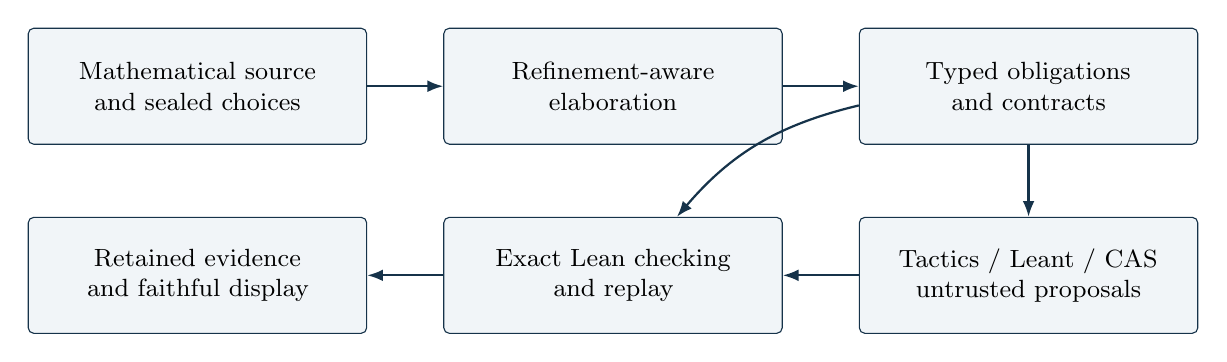
\begin{tikzpicture}[
 box/.style={draw=ink,fill=pale,rounded corners=2pt,align=center,
 text width=1.6in,minimum height=.58in,font=\small},
 arr/.style={-{Latex[length=2mm]},thick,draw=ink},node distance=.36in and .38in]
 \node[box] (source) {Mathematical source\\and sealed choices};
 \node[box,right=of source] (elab) {Refinement-aware\\elaboration};
 \node[box,right=of elab] (goals) {Typed obligations\\and contracts};
 \node[box,below=of goals] (provider) {Tactics / Leant / CAS\\untrusted proposals};
 \node[box,left=of provider] (check) {Exact Lean checking\\and replay};
 \node[box,left=of check] (out) {Retained evidence\\and faithful display};
 \draw[arr] (source)--(elab); \draw[arr] (elab)--(goals);
 \draw[arr] (goals)--(provider); \draw[arr] (provider)--(check);
 \draw[arr] (check)--(out);
 \draw[arr] (goals) to[bend right=18] (check);
\end{tikzpicture}
\caption{The proposed boundary. Provider metadata never bypasses exact checking.
The contract library supplies the mathematical theorems used by elaboration and
validation; the diagram does not imply that the frontend itself is verified.}
\end{figure}

\subsection{A rule interface that prevents accidental circularity}
A registered rule should carry an ordinary theorem whose input telescope
separates fixed data from proof obligations. Its administrative record can
contain a conclusion pattern, input-property roles, explicitly introduced data,
a cost class, and a suggested display. Only the theorem has logical authority.

The planner constructs a dependency graph in which a node can use only earlier
accepted facts or declared premises of its own continuation. Premises mentioning
newly selected output data are created after that data is bound. A topological
order prevents a common class of cyclic guard errors, but it is not a substitute
for checking the theorem term: an acyclic graph can still contain a false claim
or the wrong anchor.

The evidence index should use actual local-context identifiers and expressions.
A production implementation must not use textual variable names as proof of
identity. Renaming and alpha-equivalence can be normalized carefully; changing
a typeclass instance or a branch-local witness cannot be normalized away.

\subsection{A minimal implementation sequence}
\textbf{First, ordinary Lean contracts.} Implement the core encodings and a small
property database. Connect local positivity/nonzeroness and squarefree-level
consequences. Establish an annotated-Lean baseline before adding syntax.

\textbf{Second, one complete certificate path.} Implement the coefficient-list
operations, prove their denotation lemmas and checker soundness in Lean, and
connect reified source expressions to that denotation. Corrupt a coefficient,
misalign the multiplier arity, and alter the atom map in matched negative tests.
Theorem~\ref{thm:checker} is the mathematical specification, not a completed
Lean implementation.

\textbf{Third, local and finite observation interfaces.} Wrap the existing
local-derivative and finite-matrix theorems. Expose typed demand requests and
obligations without inventing new mathematical foundations.

\textbf{Fourth, a narrow Leant adapter.} Evaluate real property-composition and
witness-assembly obligations from those packages. The CAS can remain a provider
rather than the organizing center of the frontend.

\textbf{Fifth, syntax and display experiments.} Only after the library interface
works, add the proposed view annotations and proof-plan blocks. Measure the
additional benefit. This ordering is intentionally less ambitious than building
an independent general-purpose proof language from the outset.

\subsection{Collaboration, upgrades, and reproducibility}
A retained proof belongs to an environment, not just a source string. On a
library or toolchain upgrade, re-elaborate fixed declarations, compare their
fully elaborated statements and structure choices, and recheck the actual
axiom inventory under the destination policy. Do not reinterpret a historical
native-computation allowlist merely because a constant was renamed.

Merging branches also needs more than a line-based union of facts. If two
branches independently chose witnesses, their facts are not interchangeable.
If they prove different propositions about the same fixed object, those facts
may coexist after rechecking their context embeddings. If they merely chose
different proofs of the same proposition, the logical conflict is usually
absent, though replay metadata still needs a well-defined owner.

A semantic merge receipt should identify which mathematical objects and
contracts survived, which choices changed, and which obligations were rebuilt.
This is proposed tooling, not a guarantee that semantic merging can always be
automated.

\section{Verification status and executable companion}\label{sec:status}

\subsection{What was executed}
The accompanying \code{contract_model.py} is a standard-library Python reference
model of a \emph{small acceptance discipline}. It checks exact advertised
conclusions, backward-only dependencies, selected relation kinds, precision
weakening and differentiation loss, locality bridges, soundness plus coverage,
and collapsed bounds. It also implements integer coefficient-list addition,
convolution, and the combination checker described in
Section~\ref{sec:cas}.

The run completed with \textbf{32 passing test methods}, zero failures, and zero
errors. The archive includes the source, its console log, and a machine-readable
result record. Several test methods contain families of finite cases. The count
32 is the number of test methods, not a number of proved theorems or a directly
comparable score against another report's experiment count.

The additional arithmetic checks cover the local Frey integrality premises,
finite binomial matrices in both multiplication orders, and a shift
counterexample observation. These tests corroborate examples and catch small
implementation mistakes; the universal mathematical claims rest on the proofs
in the article, not on the finite trials.

\subsection{What the companion does not establish}
The model treats its input assumptions as already authorized. Its anchors are
stand-in identifiers, not actual Lean expressions. Its closed rule names model
theorem interfaces, not a library of kernel-checked constants. It is not a
parser for hostile input, a verified Python implementation, a secure proof
kernel, or a complete contract inference engine. In particular, successful
Python validation does not establish the truth of an input assumption.

The supplied \code{GneissCore.lean} shows ordinary-Lean encodings for properties,
behavioral composition, consequence, conditional results, respectfulness, and
complete solution predicates. It contains no \code{sorry} or added axiom in its
text, but \textbf{it was not compiled in this preparation session}, because no
Lean executable was available. It is a design specimen to compile and audit,
not an asserted kernel-verified artifact. No checker-denotation theorem is
claimed to have been completed in that Lean file.

This is a material limitation relative to the syntheses' request for a fully
proved first checker. The article supplies its mathematical proof and an
executable reference algorithm, but the end-to-end Lean implementation,
reification proof, and measured integration remain engineering deliverables.
Calling a Boolean test a formal proof would obscure exactly the distinction
the proposal is intended to enforce.

\subsection{A small acceptance-model invariant}
\begin{proposition}[Relative soundness of acyclic rule assembly]
Suppose the assumptions supplied to an assembly are true in a fixed
interpretation of its claim language, and each permitted rule preserves truth
under that interpretation. If every step references only previous entries and
its recorded conclusion is the conclusion prescribed by that rule, every
accepted entry is true in the interpretation.
\end{proposition}
\begin{proof}
Induct on the entry number. An initial entry is true by assumption. A derived
entry has only earlier premises, which are true by the induction hypothesis;
the interpreted rule's soundness makes its prescribed conclusion true. Exact
conclusion matching identifies it with the recorded entry. The last entry,
which must equal the requested target, is therefore true.
\end{proof}
This elementary proposition explains the model's design. It is deliberately
\emph{relative}: it does not establish that the Python implementation enforces
all premises for arbitrary malformed objects, or that an external assumption
was checked by Lean. A production adapter must replace those assumptions with
actual typed proof evidence and validated input structures.

\section{An adversarial suite that targets the semantics}\label{sec:negative}

The syntheses' negative catalog is a strong starting point. The relevant unit
is a matched positive and negative pair: a frontend that rejects every request
must not pass by being useless. The following table separates what the
companion tests from what remains a Lean integration obligation.

\begingroup\small
\begin{longtable}{@{}P{1.4in}P{3.37in}P{1.08in}@{}}
\toprule
Mutation & Required behavior & Current status\\
\midrule\endfirsthead
\toprule Mutation & Required behavior & Current status\\\midrule\endhead
Wrong anchor or sibling scope & Reject evidence about another variable or a fact absent from the current assumptions. & Model tests; real Lean identities pending.\\
Self-justifying guard & Reject a forward or self reference; accept an ordinary acyclic proof chain. & Model tests.\\
Overstated jet precision & Derivative of an order-$N$ observation gets order $N-1$, not $N$. & Model tests.\\
Jet presented as exact & Keep the finite guarantee; do not promote to an infinite identity. & Model tests.\\
Point equality differentiated & Require neighborhood equality; openness must match the domain on which equality holds. & Model tests.\\
Incomplete root set & Require soundness and coverage for the same predicate and candidate set. & Model tests.\\
Noncollapsed bounds & Do not infer equality from an interval with unequal endpoints; accept equal endpoints. & Model tests.\\
Wrong result target & Reject a correct fact when it is not the sealed target requested by the caller. & Model tests.\\
Certificate corruption & Reject a changed coefficient or unmatched multiplier-generator arity. & Executed coefficient tests.\\
Integer quotient cast & Require divisibility; matching printed fractions is insufficient. & Arithmetic examples; Lean bridge pending.\\
One-sided inverse on sequences & Reject finite-section transfer without causality or its equivalent presentation theorem. & Shift example; Lean adapter pending.\\
Nonunit cancellation/inversion & Separate regularity, nonzeroness, and being a unit; no silent field assumption. & Specified integration test.\\
Wrong residual-root branch & Require shared constant term and unit derivative; finite residual alone is insufficient. & Inherited counterexamples; integration pending.\\
Meaning-bearing hole & Do not let proof search choose a ring, topology, branch, or theorem parameter to ease the goal. & Specified integration test.\\
Data chosen in one branch & Do not combine a curve, level, and transfer proof from incompatible witness scopes. & Specified integration test.\\
Finite behavioral sampling & Do not certify a universal contract from passing examples or a model-relative result alone. & Specified integration test.\\
Native result without execution evidence & Algorithm correctness alone must not authorize the returned bytes. & Specified integration test.\\
Displayed edit differs from tested edit & Replay the exact displayed text from the recorded origin before marking it accepted. & Leant adapter test pending.\\
Unused false assertion & Reject publication even when a later theorem has an independent correct proof. & Frontend test pending.\\
Toolchain or structure changes & Recheck statement meaning and destination axiom policy; do not reuse a stale success badge. & Migration test pending.\\
\bottomrule
\end{longtable}
\endgroup

Many of these test families are inherited, not new discoveries
\cite{syn-a,syn-b}. The new contribution is their placement at specific
refinement and behavior-transfer rules, together with the small executed subset.
A future implementation should turn every pending row into an executable
positive/negative pair before claiming that its publication boundary is complete.

\section{Evaluation: what would make this a successful language?}\label{sec:evaluation}

\subsection{Four treatments, shared mathematics}
Use four treatments on matched tasks. The first is ordinary Lean with its
existing library and automation. The second adds the proposed contract wrappers
and property lemmas but no new surface. The third adds the same provider and
replay services through an ordinary-Lean interface. The fourth adds the
\Gneiss{} surface, inferred views, and display. This separates a good theorem
library, a good search service, and a good language interface.

All infrastructure counts. A ten-line new proof supported by a thousand-line
custom package is not compared against an unprepared Lean baseline that has
none of that package. Shared wrappers are amortized over a realistic family of
tasks, while per-task additions and maintenance are recorded separately.

\subsection{Measure more than character count}
The primary outcomes should be author interventions, elapsed active authoring
time, semantic mistakes, and comprehension of the final guarantee. Secondary
outcomes include proof replay time, memory, evidence size, dependency churn,
repair effort after a controlled edit, and the share of requests resolved by
simple lookup versus structural composition.

Character count is descriptive, not decisive. The same formula can hide a
crucial quantifier or an excluded point. A source with more visible mathematical
conditions may be the better concise proof if it removes irrelevant mechanics
without removing meaning.

For a blind reading test, ask readers to recover the exact object, domain,
branch, precision, completeness, and assumptions from a compact result before
showing its evidence expansion. Include plausible-looking negative neighbors.
Then reveal the expansion and measure whether errors are corrected. This is the
syntheses' strongest proposed usability test, and it remains central here
\cite{syn-a,syn-b}.

\subsection{Development examples are not held-out evidence}
The binomial, derivative, triangular, and FLT examples in this article are
\emph{development material}. None can subsequently be described as unseen
validation for the design shaped around it. Hold out separate theorem families,
exclude aliases and near-duplicate corollaries, and freeze those tasks before
building specialized adapters. A new filename is not sufficient evidence of
independence.

Useful controlled edits include changing an inclusive endpoint, replacing an
open domain by a nonopen one, weakening positivity to nonnegativity, changing a
coefficient ring, changing a selected algebra structure, and moving a witness
across a case boundary. The system should localize the resulting obligation
rather than silently altering the theorem or discarding the claimed proof plan.

\subsection{Stop rules and a realistic success criterion}
If the property library accounts for essentially all gains, ship that library.
If the new surface improves readability but not productivity, present it as an
explanation layer rather than a synthesis breakthrough. If inferred properties
make source meaning unpredictable, require more explicit annotations rather
than expanding default search.

The language is successful when a user can reliably state a mathematical step,
see exactly what it promises, and let the system recover routine evidence
without repeated semantic choices. It need not minimize every proof to a small
number of lines. It must make short proofs less surprising and long proofs more
modular.

\Needspace{39\baselineskip}
\section{Answers to the second synthesis's round-three questions}\label{sec:questions}

The following responses use the current second synthesis's R1--R10 labels
\cite{syn-b}. They also address the first synthesis's questions about workspace
allocation, delegation, reuse, display, and evaluation.

\begingroup\small
\begin{longtable}{@{}P{.58in}P{5.39in}@{}}
\toprule
Question & Answer in this proposal\\
\midrule\endfirsthead
\toprule Question & Answer in this proposal\\\midrule\endhead
R1 & Define executable coefficient data, prove additive and multiplicative denotation, prove checker soundness, and prove the reification bridge. Section~\ref{sec:cas} gives the mathematical proof and executable reference checker; its complete Lean formalization is explicitly still pending.\\
R2 & Treat \code{grobner} as a versioned bounded proof producer. Record its assumptions and limits; do not interpret failure as refutation or assume certificate export. Compare it with the certificate path on the same requests.\\
R3 & The evidence index points into Lean's context rather than replacing it. New state is request/dependency/display/replay accounting only when that state enables an operation not already exposed by existing Lean interfaces.\\
R4 & Preserve Lean's total operations by default for compatibility. Offer partial expressions as an explicit domain-indexed package; do not equate the two meanings through notation.\\
R5 & Begin with local property propagation and a small certified algebra path; then test locality and finite sections. This is a proposed order, not a measured winner. The already inspected cases are not held out.\\
R6 & No numerical threshold is claimed for accelerated evaluation. Measure actual data representations and workloads, with the current trust policy, before enabling it as a default.\\
R7 & Revalidate retained evidence in the destination environment and audit its actual axioms and statement interpretations. A changed axiom naming scheme is not handled by a historical blacklist.\\
R8 & Measure Leant on obligations actually generated by contracts, separating direct lemma lookup from multi-step implication, witness assembly, and relation transfer. Keep model-relative behavioral outcomes distinct.\\
R9 & Ship positive/negative pairs. The companion executes a small subset with 32 test methods; Section~\ref{sec:negative} identifies the remaining integration backlog instead of claiming the complete inherited suite passed.\\
R10 & Prefer a few implementations with distinct experimental goals over another set of broad architectural renamings. \Gneiss{} contributes one narrow organizing layer and a restricted model, not evidence that nine more proposals would improve the outcome.\\
\bottomrule
\end{longtable}
\endgroup

On the first synthesis's visibility question, the default display must expose
conditions that change the mathematical claim. On its delegation question,
a fixed relational specification may authorize data search, but routine
proof search cannot silently select meaning-bearing data. On certificate
reuse, actual entailment and context correspondence authorize reuse; neither
textual similarity nor a global strength ranking does. These are adopted
constraints, not open loopholes in the new type layer.

\section{Related work and the limits of the novelty claim}\label{sec:related}

\subsection{Refinement sorts and proof irrelevance}
Lovas and Pfenning's work on refinement types for logical frameworks studies
sort refinements and their interpretation using proof irrelevance
\cite{lovas-pfenning}. It is a direct conceptual predecessor for the separation
between a term's underlying type and additional checked properties. \Gneiss{}
therefore does not claim to invent refinement sorts, intersection-like property
views, or their proof-valued interpretation. Its proposed application is to
Lean mathematical authoring with retained object identity, behavior-directed
obligations, and observation transfer.

\subsection{Dependent specifications and effectful verification}
Dependent types already permit a function's specification to mention its input,
output, and proofs. Dijkstra monads and the F* tradition provide compositional
pre/postcondition interfaces for effects \cite{dm4free}. Current Lean
\code{mvcgen} infrastructure is an immediate implementation neighbor rather
than merely historical related work \cite{lean-mvcgen}.

The mathematical examples here differ from imperative state manipulation, but
not because they need a new logic. Their distinguishing indices are often
locality, coefficient precision, finite observations, or algebraic structure.
Those should be ordinary proposition families and theorem interfaces, with a
specialized elaboration policy rather than another foundational calculus.

\subsection{The round-two verified-CAS designs}
The certified-computation boundary, result-kind distinctions, guard scoping,
execution/reification separation, and retained proof evidence come directly
from the syntheses and their antecedent proposals \cite{syn-a,syn-b}. Demand
propagation for jets and theorem-backed result weakening are already present
there. \Gneiss{} generalizes their operational use to property-aware term
checking and explicitly analyzes the kernel-extension alternatives requested
in this round.

The proposal's novelty is therefore \emph{design integration and a concrete
elaboration discipline}, not a new foundational theorem about dependent types,
a newly discovered matrix theorem, or the first idea of checking CAS results.
The real novelty claim would become stronger only after an implementation
shows that these pieces interact more effectively than their separate Lean
counterparts.

\section{Conclusion: make the mathematical type carry the useful information}

A concise proof language should not ask the kernel to guess what a mathematician
meant. It should ask the author for the mathematical objects, relevant
assumptions, and conceptual steps, and then reconstruct the routine evidence
that connects those steps. The reconstruction should be guided by richer
\emph{mathematical types}: contextual properties of selected terms and
behavioral contracts of the operations that consume them.

\Gneiss{} proposes ordinary Lean carriers with proof-valued views; dependent,
input/output behavioral specifications; theorem-backed observation transfer;
and bounded bidirectional elaboration whose output is ordinary Lean evidence.
This makes positivity available without renaming a number, locality available
without globalizing an analytic hypothesis, finite sections available without
misapplying a finite-dimensional theorem, and witness-local laws available
without conflating the witnesses themselves.

The first kernel should remain Lean's existing kernel. A genuine refinement
primitive is a possible later engineering experiment, not the premise of the
design. The first deliverables should be a small contract library, one complete
Lean checker/reification path, and a narrow property-aware elaborator tested
against an equally equipped Lean baseline. The paper proofs and executed
reference model supplied here make that agenda more concrete, while leaving
its uncompleted formalization and empirical claims plainly visible.

The desired compression is not ``omit whatever the checker will tolerate.''
It is \emph{retain the mathematical distinctions, infer the routine consequences,
and make the relationship between the two explicit enough to verify}.

\appendix
\section{A compact grammar and its intended restrictions}\label{app:grammar}

This grammar sketches the surface needed by the examples. It is not a complete
parser specification and has no claimed implementation.
\begin{lstlisting}
view       ::= carrier ["with" property ("and" property)*]
binder     ::= name ":" view
             | name ":" carrier "where" proposition
statement  ::= "assume" name ":" proposition
             | "let" name ":=" term ["with" property*]
             | "know" term ":" view
             | "have" name ":" proposition "by" method
             | "obtain" binders "by" method "retaining" contracts
             | "show" proposition "by" plan
contract   ::= "requires" proposition
             | "ensures" proposition
             | "respects" relation "into" relation
method     ::= registered-method ["using" evidence*]
             | explicit-lean-proof
             | "search" provider-profile
\end{lstlisting}
The parser may infer punctuation and conventional mathematical notation, but
not quantifier dependencies or meaning-bearing structures from a successful
proof search. \code{know} requires accepted evidence; \code{assume} is an explicit
hypothesis or branch introduction; \code{obtain} declares selected data and
scopes its dependent properties. A registered method is a theorem interface,
not a free-form natural-language promise.

The initial implementation should omit automatic generalization of theorem
headers, unrestricted implicit coercions between observation relations, and
unconstrained natural-language parsing. These omissions reduce ambiguity while
leaving the central property and behavior inference experiment intact.

\section{Source register and reproducibility}\label{app:sources}

\subsection{Pinned repositories}
All four repository heads below were inspected directly. The retrieval date was
6 September 2026. Full commit identifiers, rather than moving branch names,
identify the reading snapshot.
\begin{description}[style=nextline]
\item[Brainstorm]
\code{b052ec011beb96a7c48df2a9988823f0f779b445}.
Both requested round-two syntheses. Their respective file blob identifiers were
\code{ae7c21dac1ba615e36dff07ea6f6a1c433a40108} and
\code{de10daae20af19285ee07a476caa94e577f7d7d9}.
\item[ProveIt]
\code{24ce8bd743eaab64a91ce90725ea00f498d319d2}.
Read the binomial-inversion development through its module-valued interface,
the local autonomous-derivative file, and the triangular-kernel inverse file.
\item[Fermat's Last Theorem]
\code{aa2d8b34692b16c70f699536de0d8e75b9a3e9ef}.
Read README and proof path, the Frey-package definition, and the
semistable-model modularity proof's configuration and mathematical body. Its
README specifies Lean 4.33.1 and Mathlib v4.33.0; those full builds were not rerun.
\item[Leant]
\code{3a40904be8a410d832d9ab6900b3d3e7b425eccb}.
Read the full verification boundary, the engine interface/header, and the
current detailed synthesis documentation's semantic-origin, verification,
Length-handoff, and problem-sealing discussion. This was a boundary review,
not a complete audit or rerun of Leant's test corpus.
\end{description}

\subsection{Archive contents and build instructions}
\begin{lstlisting}
gneiss.tex              Self-contained article source and bibliography
gneiss.pdf              Compiled article
GneissCore.lean          Uncompiled ordinary-Lean design specimen
contract_model.py       Executed acceptance/reference-algebra model
tests.log               Verbatim test console output
test_results.json       Test-method counts and explicit scope limitations
sources.json            Machine-readable repository/source register
validation.json         Build, test, and visual-review status
README.md               Build and verification-status notes
build.sh                LaTeX build command
SHA256SUMS              Integrity hashes for the delivered files
\end{lstlisting}
To rebuild the article, run \code{latexmk -pdf gneiss.tex} in an environment with
the standard TeX packages used in the preamble. To rerun the reference model,
run \code{python3 contract_model.py}. To assess the Lean specimen, first select
and record a Lean toolchain, compile it, and inspect its actual axiom reports.
A text search for forbidden words is not a replacement for that process.

\subsection{A final distinction about evidence}
The PDF compilation and Python tests are activities performed for this article.
The cited repositories' Lean experiments and large proof-verification results
are source-reported activities. Theorems in the main text have mathematical
proofs given in the article. The proposed frontend, the complete Lean
polynomial checker, and the claimed authoring improvements remain unimplemented
or unmeasured. These categories should stay separate when this proposal is
merged into a later synthesis.

\begin{thebibliography}{99}
\small\raggedright
\setlength{\itemsep}{3pt}
\setlength{\parskip}{0pt}
\bibitem{syn-a}
Codex. \emph{Mathematical Objects, Certified Computation: A Unified Evaluation
of Nine Proof-Language Proposals}. Round-two synthesis, revised September 2026.
Brainstorm, pinned commit \code{b052ec01}.
\url{https://github.com/VladimirReshetnikov/Brainstorm/blob/b052ec011beb96a7c48df2a9988823f0f779b445/docs/round-2/synthesis/unified-report.tex}.

\bibitem{syn-b}
Claude. \emph{Nine Workbenches: Certified Computation in a Mathematician's Proof
Language over Lean}. Round-two synthesis, 5 September 2026, revised 6 September.
Brainstorm, pinned commit \code{b052ec01}.
\url{https://github.com/VladimirReshetnikov/Brainstorm/blob/b052ec011beb96a7c48df2a9988823f0f779b445/docs/round-2/unified_report/unified_report.tex}.

\bibitem{binomial}
V. Reshetnikov and contributors. \emph{BinomialInversion.lean}. ProveIt,
commit \code{24ce8bd7}, especially the kernel orthogonality and additive-group
inversion interfaces.
\url{https://github.com/VladimirReshetnikov/ProveIt/blob/24ce8bd743eaab64a91ce90725ea00f498d319d2/Analysis/FabiusFunction/Lean/FabiusFunction/BinomialInversion.lean}.

\bibitem{autonomous}
V. Reshetnikov and contributors. \emph{AutonomousIteratedDeriv.lean}. ProveIt,
commit \code{24ce8bd7}, theorem \code{AutonomousODE.iteratedDeriv_eq_comp}.
\url{https://github.com/VladimirReshetnikov/ProveIt/blob/24ce8bd743eaab64a91ce90725ea00f498d319d2/Analysis/FabiusFunction/Lean/FabiusFunction/AutonomousIteratedDeriv.lean}.

\bibitem{triangular}
V. Reshetnikov and contributors. \emph{TriangularKernelInverse.lean}. ProveIt,
commit \code{24ce8bd7}, especially \code{kernelMatrix_mul_apply} and
\code{lowerTriangular_orthogonal_comm}.
\url{https://github.com/VladimirReshetnikov/ProveIt/blob/24ce8bd743eaab64a91ce90725ea00f498d319d2/Analysis/FabiusFunction/Lean/FabiusFunction/TriangularKernelInverse.lean}.

\bibitem{flt-readme}
Anthropic and credited upstream contributors. \emph{Fermat's Last Theorem in
Lean 4}, README, commit \code{aa2d8b34}, 3 September 2026.
\url{https://github.com/anthropics/fermats-last-theorem/blob/aa2d8b34692b16c70f699536de0d8e75b9a3e9ef/README.md}.

\bibitem{flt-path}
Anthropic and credited upstream contributors. \emph{The route of the proof},
\code{PROOF-PATH.md}, commit \code{aa2d8b34}.
\url{https://github.com/anthropics/fermats-last-theorem/blob/aa2d8b34692b16c70f699536de0d8e75b9a3e9ef/PROOF-PATH.md}.

\bibitem{frey-package}
K. Buzzard, R. Van de Velde, P. Monticone, and contributors; ported in the
Anthropic repository. \emph{Def\_FLTPrelim\_FreyPackage.lean}, commit
\code{aa2d8b34}. Source notice credits the Imperial College London FLT project.
\url{https://github.com/anthropics/fermats-last-theorem/blob/aa2d8b34692b16c70f699536de0d8e75b9a3e9ef/Definitions/Def_FLTPrelim_FreyPackage.lean}.

\bibitem{flt-modularity}
Anthropic and credited upstream contributors.
\emph{S\_WeierstrassCurve\_modularity\_of\_semistableModel.lean},
commit \code{aa2d8b34}, especially lines 140--211.
\url{https://github.com/anthropics/fermats-last-theorem/blob/aa2d8b34692b16c70f699536de0d8e75b9a3e9ef/P2M/Sol/S_WeierstrassCurve_modularity_of_semistableModel.lean}.

\bibitem{leant-verification}
V. Reshetnikov and contributors. \emph{Leant.Synth.Verification},
commit \code{3a40904b}.
\url{https://github.com/VladimirReshetnikov/Leant/blob/3a40904be8a410d832d9ab6900b3d3e7b425eccb/src/Leant/Synth/Verification.hs}.

\bibitem{leant-engine}
V. Reshetnikov and contributors. \emph{Leant.Synth.Engine}, interface and
boundary documentation, commit \code{3a40904b}.
\url{https://github.com/VladimirReshetnikov/Leant/blob/3a40904be8a410d832d9ab6900b3d3e7b425eccb/src/Leant/Synth/Engine.hs}.

\bibitem{leant-internals}
V. Reshetnikov and contributors. \emph{\texttt{:synth} internals}, semantic
origins, exact-text verification, Length handoff and problem sealing,
commit \code{3a40904b}.
\url{https://github.com/VladimirReshetnikov/Leant/blob/3a40904be8a410d832d9ab6900b3d3e7b425eccb/docs/synth-internals.md}.

\bibitem{lean-subtypes}
Lean team. \emph{Subtypes}. The Lean Language Reference, accessed 6 September
2026. \url{https://lean-lang.org/doc/reference/latest/Basic-Types/Subtypes/}.

\bibitem{lean-types}
Lean team. \emph{The Type System}. The Lean Language Reference, accessed
6 September 2026.
\url{https://lean-lang.org/doc/reference/latest/The-Type-System/}.

\bibitem{lean-validation}
Lean team. \emph{Validating a Lean Proof}. The Lean Language Reference, accessed
6 September 2026.
\url{https://lean-lang.org/doc/reference/latest/ValidatingProofs/}.

\bibitem{lean-mvcgen}
Lean team. \emph{Verifying Imperative Programs Using mvcgen}. Lean tutorials,
accessed 6 September 2026.
\url{https://lean-lang.org/doc/tutorials/latest/mvcgen/}.

\bibitem{lean-mvcgen-enabling}
Lean team. \emph{Enabling mvcgen For Monads}. The Lean Language Reference,
accessed 6 September 2026.
\url{https://lean-lang.org/doc/reference/latest/The--mvcgen--tactic/Enabling--mvcgen--For-Monads/}.

\bibitem{lovas-pfenning}
W. Lovas and F. Pfenning. \emph{Refinement Types for Logical Frameworks and
Their Interpretation as Proof Irrelevance}. arXiv:1009.1861, 2010.
\url{https://arxiv.org/abs/1009.1861}.

\bibitem{dm4free}
D. Ahman, C. Hri\c{t}cu, K. Maillard, G. Mart\'inez, G. Plotkin,
J. Protzenko, A. Rastogi, and N. Swamy. \emph{Dijkstra Monads for Free}.
POPL 2017; author-maintained project page and abstract.
\url{https://fstar-lang.org/papers/dm4free/}.
\end{thebibliography}
\end{document}
